\documentclass[11pt,a4paper]{article}
\usepackage[utf8]{inputenc}
\usepackage[T1]{fontenc}
\usepackage[margin=2.5cm]{geometry}
\usepackage{amsmath,amsthm,amssymb,mathtools}
\usepackage{enumitem}
\usepackage{hyperref}
\usepackage{cleveref}
\usepackage{booktabs}
\usepackage{array}
\usepackage{xcolor}
\usepackage{listings}
\usepackage[ruled,vlined,linesnumbered]{algorithm2e}
\usepackage{tikz-cd}
\usepackage{graphicx}
\usepackage{natbib}
\usepackage{authblk}
\graphicspath{{figures/}}

\theoremstyle{plain}
\newtheorem{theorem}{Theorem}[section]
\newtheorem{proposition}[theorem]{Proposition}
\newtheorem{lemma}[theorem]{Lemma}
\newtheorem{corollary}[theorem]{Corollary}
\newtheorem{conjecture}[theorem]{Conjecture}
\theoremstyle{definition}
\newtheorem{definition}[theorem]{Definition}
\newtheorem{example}[theorem]{Example}
\theoremstyle{remark}
\newtheorem{remark}[theorem]{Remark}

\newcommand{\R}{\mathbb{R}}
\newcommand{\C}{\mathbb{C}}
\newcommand{\cF}{\mathcal{F}}
\newcommand{\cO}{\mathcal{O}}
\newcommand{\cX}{\mathcal{X}}
\newcommand{\cA}{\mathcal{A}}
\newcommand{\cS}{\mathcal{S}}
\newcommand{\cT}{\mathcal{T}}
\newcommand{\cG}{\mathcal{G}}
\newcommand{\cL}{\mathcal{L}}
\newcommand{\cH}{\mathcal{H}}
\newcommand{\cD}{\mathcal{D}}
\newcommand{\cB}{\mathcal{B}}
\newcommand{\cP}{\mathcal{P}}
\newcommand{\cN}{\mathcal{N}}
\newcommand{\cE}{\mathcal{E}}
\newcommand{\fU}{\mathfrak{U}}
\newcommand{\Attn}{\mathrm{Attn}}
\newcommand{\Res}{\mathrm{Res}}
\newcommand{\tr}{\mathrm{tr}}
\newcommand{\im}{\mathrm{im}}
\newcommand{\Hcoh}{\mathcal{H}_{\mathrm{coh}}}
\newcommand{\Cech}{\check{C}}
\newcommand{\CechH}{\check{H}}
\DeclareMathOperator{\rank}{rank}
\DeclareMathOperator{\softmax}{softmax}

\lstset{
  basicstyle=\ttfamily\small,
  keywordstyle=\color{blue!70!black}\bfseries,
  commentstyle=\color{green!50!black}\itshape,
  numbers=left, numberstyle=\tiny\color{gray},
  breaklines=true, frame=single, framerule=0.4pt,
  rulecolor=\color{gray!50}, backgroundcolor=\color{gray!5},
  language=Python
}

\hypersetup{
  colorlinks=true, linkcolor=blue!70!black,
  citecolor=green!50!black, urlcolor=red!60!black,
  pdftitle={Sheaf-Theoretic Foundations for Transformer Architectures},
  pdfauthor={Ayman Machhidan}
}

\title{\textbf{Sheaf-Theoretic Foundations for Transformer Architectures:}\\[0.3em]
\large A Holomorphic Approach via Spectral Theory}
\author{Ayman Machhidan}
\date{\today}

\begin{document}
\maketitle

\begin{abstract}
We introduce a rigorous sheaf-theoretic framework for Transformer architectures, termed \textbf{Sheaf Transformers} ($\cS$-Transformers), in which attention mechanisms are recast as section-restriction operations on sheaves defined over topological spaces of token representations. By equipping these sheaves with holomorphic structure via barycentric rational interpolation, we establish connections between self-attention, complex analysis, and spectral theory. We prove that standard softmax attention fails to be a sheaf morphism (Theorem~\ref{thm:softmax-failure}), that holomorphic attention with meromorphic kernels restores this property under explicit conditions (Theorem~\ref{thm:hol-morphism}), and we provide a computable hallucination cohomology index $\Hcoh$ with polynomial-time algorithms. We further extend the framework in two directions toward artificial general intelligence: (1)~a \textbf{temporal belief sheaf} for long-term memory, where the condition $E_{\mathrm{mem}} = 0$ characterizes narrative coherence and sheaf diffusion provably converges to coherent belief states (Theorem~\ref{thm:belief-propagation}); and (2)~a \textbf{multi-agent sheaf intelligence} framework, where the cohomological dimension $\dim\CechH^1$ provides a communication complexity lower bound for consensus (Theorem~\ref{thm:comm-complexity}). A spectral generalization bound via the sheaf Laplacian accompanies the theory. We validate the framework experimentally on synthetic data: $\Hcoh$ achieves perfect hallucination detection (AUROC $= 1.0$) while attention entropy fails (AUROC $\approx 0.5$); the gluing layer achieves 100\% cocycle reduction; and sheaf diffusion converges exponentially in both multi-agent and temporal memory settings.
\end{abstract}

\noindent\textbf{Keywords:} Sheaf theory, Transformer, attention, cohomology, spectral graph theory, hallucination detection, temporal memory, multi-agent systems, narrative coherence.

\tableofcontents
\newpage

%% ============================================================
\section{Introduction}\label{sec:intro}

\subsection{Motivation}
Modern Transformer architectures~\citep{vaswani2017} suffer from quadratic attention complexity, hallucination, poor long-range coherence, and opacity. We propose that \textbf{sheaf theory} provides the natural language for understanding and improving Transformers. The central insight is:

\begin{quote}
\emph{Self-attention is a recollement problem: assembling coherent global representations from local contextual data, subject to compatibility conditions.}
\end{quote}

\subsection{Why Holomorphic Sheaves?}
Holomorphic sheaves offer: (i)~\textbf{rigidity on thickenings}: by embedding discrete tokens into open complex domains $U^\sharp$ (Definition~\ref{def:hol-sheaf}), analytic continuation provides genuine rigidity unavailable on finite sets; (ii)~\textbf{spectral theory} for representation quality analysis; (iii)~\textbf{computational tractability} via residue calculus. The passage from discrete tokens to continuous domains uses barycentric rational interpolation~\citep{berrut2004}, avoiding the Runge phenomenon (\S\ref{sec:interpolation}).

\subsection{Related Work}
\citet{hansen2020} introduced sheaf neural networks on graphs. \citet{bodnar2022} developed neural sheaf diffusion for GNNs. \citet{weiss2021} analyzed Transformers algebraically. Our framework extends sheaf methods to Transformers with a geometric perspective.

\subsection{Contributions}
\begin{enumerate}[nosep]
\item Theorem~\ref{thm:softmax-failure}: softmax attention is \emph{not} a sheaf morphism, with explicit quantification.
\item The hallucination cohomology index $\Hcoh$ (\S\ref{sec:cohomology}).
\item Theorem~\ref{thm:hol-morphism}: holomorphic attention \emph{is} a sheaf morphism under stated conditions.
\item Spectral generalization bounds via the sheaf Laplacian (Theorem~\ref{thm:generalization}).
\item Temporal belief sheaf for long-term memory with narrative coherence (Theorems~\ref{thm:coherent-update},~\ref{thm:narrative},~\ref{thm:belief-propagation}).
\item Multi-agent sheaf intelligence with communication complexity lower bound (Theorems~\ref{thm:consensus},~\ref{thm:comm-complexity},~\ref{thm:consensus-convergence}).
\item Complete experimental protocol (\S\ref{sec:experiments}).
\end{enumerate}

%% ============================================================
\section{Mathematical Foundations}\label{sec:foundations}

\subsection{The Attention Topology}

\begin{definition}[Attention Topology]\label{def:attn-topology}
Given attention matrix $A \in \R^{n \times n}$ with $a_{ij} \geq 0$ and threshold $\epsilon > 0$, the \textbf{attention neighborhood} of $x_i$ is $N_\epsilon(x_i) = \{x_j \in \cX_n \mid a_{ij} > \epsilon\}$. The attention topology $\tau_A$ is generated by $\mathcal{B} = \{N_\epsilon(x_i)\} \cup \{\emptyset, \cX_n\}$.
\end{definition}

\begin{proposition}\label{prop:attn-topology}
(i) If all $a_{ij} > \epsilon$, then $\tau_A$ is indiscrete. (ii)~If $A$ is block-diagonal with blocks $B_1, \ldots, B_m$, then each $B_k$ is clopen. (iii)~Connected components correspond to maximal attention communities.
\end{proposition}

\begin{proof}
(i) $N_\epsilon(x_i) = \cX_n$ for all $i$, so only $\emptyset$ and $\cX_n$ are open. (ii) For $x_i \in B_k$ and $x_j \notin B_k$, $a_{ij} = 0$, so $N_\epsilon(x_i) \subseteq B_k$. Each $B_k$ is open; as the complement of a union of other open blocks, it is also closed. (iii) In the finite Alexandrov topology, connectedness is equivalent to path-connectedness via above-threshold attention links.
\end{proof}

\subsection{The Cellular Representation Sheaf}

\paragraph{Attention graph.}
Let $G_A = (\cX_n, E_A)$ be the attention graph, where $(i,j) \in E_A$ iff $a_{ij} > \epsilon$ (or the attention mask permits interaction). This is the $1$-skeleton of the nerve of the cover $\{N_\epsilon(x_i)\}$.

\begin{definition}[Cellular Representation Sheaf]\label{def:rep-sheaf}
A \textbf{(cellular) representation sheaf} $\cF$ on the attention graph $G_A$ assigns:
\begin{enumerate}[label=(\roman*),nosep]
\item A \textbf{stalk} $\cF_i \cong \R^d$ to each node $i \in \cX_n$ (token embedding space).
\item A \textbf{constraint stalk} $\cF_{ij} \cong \R^{d_e}$ to each edge $(i,j) \in E_A$ (overlap/compatibility space, with $d_e \leq d$).
\item \textbf{Restriction maps} $\rho_{i \to ij}: \cF_i \to \cF_{ij}$ and $\rho_{j \to ij}: \cF_j \to \cF_{ij}$ (linear maps encoding semantic compatibility constraints between tokens $i$ and~$j$).
\end{enumerate}
A \textbf{global section} is a collection $s = (s_i)_{i \in \cX_n}$, $s_i \in \cF_i$, such that $\rho_{i \to ij}(s_i) = \rho_{j \to ij}(s_j)$ for every edge $(i,j) \in E_A$.

In the attention context, we set $d_e = d$ and parameterize $\rho_{i \to ij} = W_{ij}^{(L)} \in \R^{d \times d}$, $\rho_{j \to ij} = W_{ij}^{(R)} \in \R^{d \times d}$, where these matrices are functions of the attention weights (e.g., $W_{ij}^{(L)} = \alpha_{ij}^{1/2} I_d$ or learned linear maps).
\end{definition}

\begin{remark}[Why nontrivial restriction maps matter]\label{rem:nontrivial-sheaf}
If all restriction maps were coordinate projections ($\rho_{i \to ij} = \rho_{j \to ij} = \mathrm{id}$), the sheaf would be the \emph{constant sheaf}, for which $\CechH^1 = 0$ generically and no obstruction to gluing arises. The power of the cellular sheaf framework lies in the \textbf{nontrivial} restriction maps: different heads may ``project'' a token's representation into \emph{different compatibility subspaces}, and it is the failure of these projections to agree that produces nonzero $\CechH^1$. This is the precise sense in which ``locally coherent'' head outputs fail to glue globally---hallucination corresponds to irreconcilable compatibility constraints across the attention graph.
\end{remark}

\subsection{Attention as a Sheaf Morphism}\label{sec:attn-morphism}

\begin{definition}\label{def:attn-morphism}
The attention at layer $\ell$ on open set $U$ is:
\[
\Attn_U^{(\ell)}(s)_i = \sum_{j: x_j \in U} \alpha_{ij}^{(U)} (h_j W_V), \quad
\alpha_{ij}^{(U)} = \frac{\exp(s_{ij})}{\sum_{k \in U} \exp(s_{ik})},
\]
where $s_{ij} = (h_i W_Q)(h_j W_K)^\top / \sqrt{d_k}$.
\end{definition}

\begin{theorem}[Failure of Sheaf Morphism]\label{thm:softmax-failure}
Standard softmax attention is \textbf{not} a sheaf morphism. The commutativity $\rho_{V,U} \circ \Attn_V = \Attn_U \circ \rho_{V,U}$ fails whenever $U \subsetneq V$ and tokens in $U$ attend to tokens in $V \setminus U$.
\end{theorem}

\begin{proof}
For $x_i \in U$, let $Z_V = \sum_{k \in V} e^{s_{ik}}$ and $Z_U = \sum_{k \in U} e^{s_{ik}}$. Since $U \subsetneq V$, $Z_V > Z_U$.

\textbf{Left side} (attention in $V$, restrict to $U$):
\[
[\rho_{V,U} \circ \Attn_V(s)]_i = \sum_{j \in U} \frac{e^{s_{ij}}}{Z_V}(h_j W_V) + \sum_{j \in V \setminus U} \frac{e^{s_{ij}}}{Z_V}(h_j W_V).
\]

\textbf{Right side} (restrict, then attention in $U$):
\[
[\Attn_U \circ \rho_{V,U}(s)]_i = \sum_{j \in U} \frac{e^{s_{ij}}}{Z_U}(h_j W_V).
\]

The discrepancy is:
\[
\Delta_i = \sum_{j \in U}\Bigl(\frac{e^{s_{ij}}}{Z_V} - \frac{e^{s_{ij}}}{Z_U}\Bigr)(h_j W_V) + \sum_{j \in V \setminus U} \frac{e^{s_{ij}}}{Z_V}(h_j W_V).
\]
Let $p_i = \sum_{j \in V \setminus U} \alpha_{ij}^{(V)}$. Then $\|\Delta_i\| \leq p_i(\max_V \|h_j W_V\| + \max_U \|h_j W_V\|)$, vanishing iff $p_i = 0$.
\end{proof}

\begin{corollary}[When Softmax Becomes Natural]\label{cor:block-diagonal}
If attention uses a \textbf{hard mask} $M_{ij} \in \{0, -\infty\}$ so that $s_{ij} = -\infty$ for forbidden pairs, then masked softmax attention defines a sheaf morphism on the induced subgraph iff the mask makes each open set $U$ \emph{attention-closed}: no node in $U$ attends to nodes in $V \setminus U$. In matrix terms, this holds iff $A$ is block-diagonal with $U$ as a union of blocks.
\end{corollary}

\begin{proof}
By Theorem~\ref{thm:softmax-failure}, the discrepancy $\Delta_i = 0$ for all $x_i \in U$ iff $p_i = \sum_{j \in V \setminus U} \alpha_{ij}^{(V)} = 0$ for all~$x_i \in U$. In standard (unmasked) softmax, $\alpha_{ij}^{(V)} = e^{s_{ij}}/Z_V > 0$ for all pairs, so $p_i = 0$ is impossible unless $U = V$. With hard masking, $s_{ij} = -\infty$ gives $e^{s_{ij}} = 0$, so $p_i = 0$ whenever $M_{ij} = -\infty$ for all $j \in V \setminus U$, i.e., $U$ is attention-closed. Since this must hold for every pair $U \subseteq V$ in the open cover, $A$ must be block-diagonal.
\end{proof}

\begin{remark}\label{rem:masking-practice}
In practice, attention-closure is approximated by causal masking (autoregressive models), sliding-window attention (Longformer), or block-sparse patterns (BigBird). Our framework provides a sheaf-theoretic \emph{reason} why these structural restrictions improve coherence: they create sub-covers on which softmax \emph{is} a sheaf morphism.
\end{remark}

%% ============================================================
\section{Holomorphic Structure}\label{sec:holomorphic}

\subsection{Interpolation Framework}\label{sec:interpolation}

\begin{definition}\label{def:complex-pos}
A \textbf{complex position embedding} is an injective $\phi: \cX_n \to \C$, $x_i \mapsto z_i$, with $|z_i - z_j| \geq \delta > 0$.
\end{definition}

\begin{proposition}[Barycentric Rational Interpolation]\label{prop:barycentric}
For distinct $z_i \in \C$ and $h_i \in \C^d$, the interpolant
\[
f(z) = \sum_{i=1}^n h_i \cdot \ell_i(z), \quad \ell_i(z) = \frac{\omega_i/(z - z_i)}{\sum_j \omega_j/(z - z_j)}, \quad \omega_i = \prod_{j \neq i}(z_i - z_j)^{-1},
\]
satisfies $f(z_i) = h_i$, is meromorphic on $\C \setminus \{z_i\}$, and avoids the Runge phenomenon.
\end{proposition}

\begin{proof}
The function $f(z) = N(z)/D(z)$ where $N(z) = \sum_i \omega_i h_i/(z - z_i)$ and $D(z) = \sum_j \omega_j/(z - z_j)$. Both $N$ and $D$ are meromorphic with simple poles at each~$z_i$.

\textbf{Interpolation.} At $z = z_i$, multiply numerator and denominator by $(z - z_i)$: $\lim_{z \to z_i} (z - z_i)N(z) = \omega_i h_i$ and $\lim_{z \to z_i}(z-z_i)D(z) = \omega_i$. By L'H\^{o}pital's rule, $f(z_i) = \omega_i h_i / \omega_i = h_i$.

\textbf{Meromorphicity.} Away from the~$z_i$, both $N$ and $D$ are holomorphic. Poles of $f$ occur only where $D(z) = 0$ and $N(z) \neq 0$, giving at most $n-1$ poles (the degree of the polynomial $\prod_j(z - z_j) \cdot D(z)$).

\textbf{Avoidance of Runge phenomenon.} Unlike Lagrange polynomial interpolation (degree~$n-1$), the barycentric rational form has numerator and denominator of degree~$\leq n-1$, yielding a rational function of type~$(n-1, n-1)$. By~\citet{floater2007}, Theorem~2.1, for Floater--Hormann weights with blending parameter~$d_{\mathrm{blend}} \geq 1$, the interpolant has no real poles and achieves approximation order $O(h^{d_{\mathrm{blend}}+1})$ where $h$ is the mesh spacing, without the exponential growth that characterizes Runge's phenomenon.
\end{proof}

\begin{definition}[Token Thickening and Holomorphic Sheaf]\label{def:hol-sheaf}
Fix a complex position embedding $\phi: \cX_n \to \C$ (Definition~\ref{def:complex-pos}). For a thickening radius $r > 0$ with $r < \delta/2$ (where $\delta = \min_{i \neq j}|z_i - z_j|$), define the \textbf{connected thickened domain} of $U \subseteq \cX_n$ as:
\[
U^\sharp := \bigcup_{x_i \in U} D(z_i, r) \;\cup\; \bigcup_{(i,j) \in E_A(U)} \mathrm{tube}(z_i, z_j, r/2),
\]
where $D(z_i, r) = \{w \in \C : |w - z_i| < r\}$ is an open disc and $\mathrm{tube}(z_i, z_j, r/2) = \{w \in \C : \mathrm{dist}(w, [z_i, z_j]) < r/2\}$ is an open tubular neighborhood of the line segment $[z_i, z_j]$, with $E_A(U) = \{(i,j) \in E_A : x_i, x_j \in U\}$ the attention edges restricted to~$U$.

The \textbf{holomorphic sheaf} $\cO_\cX$ assigns:
\[
\cO_\cX(U) := \{f : U^\sharp \to \C^d \mid f \text{ holomorphic on } U^\sharp\},
\]
with restriction by ordinary restriction of holomorphic functions: $\rho_{V,U}: \cO_\cX(V) \to \cO_\cX(U)$ sends $f \mapsto f|_{U^\sharp}$.
\end{definition}

\begin{proposition}\label{prop:hol-is-sheaf}
$\cO_\cX$ is a sheaf on $(\cX_n, \tau_A)$.
\end{proposition}

\begin{proof}
Each $U^\sharp$ is an open subset of~$\C$, and if $U$ spans a connected component of the attention graph $G_A$, then $U^\sharp$ is connected (the tubes provide paths between discs). \textbf{Locality}: functions agreeing on each $U_\alpha^\sharp$ agree on $U^\sharp = \bigcup_\alpha U_\alpha^\sharp$. \textbf{Gluing}: compatible holomorphic functions $f_\alpha \in \cO_\cX(U_\alpha)$ agree on the overlaps $(U_\alpha \cap U_\beta)^\sharp$, which are \emph{connected open} subsets of~$\C$. By the identity theorem for holomorphic functions on connected open sets, the $f_\alpha$ glue to a unique $f \in \cO_\cX(U)$.
\end{proof}

\begin{remark}[Why connected thickening matters]\label{rem:thickening}
Without tubes, the thickened domain would be a disjoint union of discs, providing no inter-token holomorphic rigidity: a function could take arbitrary independent values on each disc. The tubes enforce \textbf{analytic continuation between tokens}: if $f$ is holomorphic on $U^\sharp$ and known on $D(z_i, r)$, its values on $D(z_j, r)$ are determined whenever $z_i$ and $z_j$ are connected by attention-edge tubes. This is the precise mechanism through which holomorphic structure creates ``context sensitivity.'' The interpolant $f_s$ of Proposition~\ref{prop:barycentric} is meromorphic on~$\C$; since $r < \delta/2$, no poles of $f_s$ lie in the discs, and $f_s$ extends holomorphically to the tubes (which lie in the pole-free region). Thus $f_s|_{U^\sharp} \in \cO_\cX(U)$.
\end{remark}

\subsection{Meromorphic Attention Kernel}

\begin{definition}\label{def:kernel}
The \textbf{meromorphic kernel} is $K_\lambda(z_i, z_j) = [(z_i - z_j)^2 + \lambda^2]^{-1}$, $\lambda > 0$.
\end{definition}

\begin{proposition}\label{prop:kernel}
(i) $K_\lambda$ has simple poles at $z_j = z_i \pm i\lambda$. (ii)~$\Res_{z_j = z_i + i\lambda} K_\lambda = (2i\lambda)^{-1}$. (iii)~On $\R$, $K_\lambda > 0$ and decays as $O(|z_i - z_j|^{-2})$. (iv)~$K_\lambda$ is the Poisson kernel at height $\lambda$ (up to normalization).
\end{proposition}

\begin{proof}
(i) Factor: $K_\lambda = [(z_i - z_j - i\lambda)(z_i - z_j + i\lambda)]^{-1}$. (ii) Standard residue computation. (iii) Denominator positive on $\R$. (iv) $P_\lambda(x) = \lambda/[\pi(x^2 + \lambda^2)] = (\lambda/\pi) K_\lambda(0,x)$.
\end{proof}

\subsection{Holomorphic Attention}

\begin{definition}[Sub-Sheaf of Extendable Sections]\label{def:ext-sheaf}
Define the \textbf{sub-sheaf of globally extendable sections} $\cO_\cX^{\mathrm{ext}} \subseteq \cO_\cX$ by:
\[
\cO_\cX^{\mathrm{ext}}(U) := \{f|_{U^\sharp} : f \in \cO_\cX(\cX_n) \text{ is a global section restricting to } U\}.
\]
Elements of $\cO_\cX^{\mathrm{ext}}(U)$ are restrictions of holomorphic functions defined on the full thickened domain $\cX_n^\sharp$. Restrictions are inherited: $\rho_{V,U}: \cO_\cX^{\mathrm{ext}}(V) \to \cO_\cX^{\mathrm{ext}}(U)$ sends $f|_{V^\sharp} \mapsto f|_{U^\sharp}$.
\end{definition}

\begin{remark}\label{rem:ext-sheaf}
In the Transformer setting, $\cO_\cX^{\mathrm{ext}}$ is the natural domain: the barycentric interpolant $f_s$ is always computed from the full input sequence (all tokens), producing a global holomorphic function that is then evaluated locally. This matches the computational reality of self-attention, where each token has access to the entire context.
\end{remark}

\begin{definition}[Global Holomorphic Attention]\label{def:hol-attn}
Let $\Gamma_X$ be a \textbf{fixed} contour enclosing $\{z_j \pm i\lambda : j \in \cX_n\}$ (all poles of $K_\lambda$ for all token pairs). For a section $s$ with holomorphic interpolant $f_s \in \cO_\cX^{\mathrm{ext}}(\cX_n)$:
\begin{equation}\label{eq:hol-attn}
\cA_{\mathrm{hol}}(s)_i = \frac{1}{2\pi i}\oint_{\Gamma_X} \frac{f_s(w) \cdot g_i(w)}{(z_i - w)^2 + \lambda^2}\,dw,
\end{equation}
where $g_i(w) = (h_i W_Q)(f_s(w) W_K)^\top / \sqrt{d_k}$ and $\Gamma_X$ is the \textbf{same contour for all open sets~$U$}. For $U \subseteq \cX_n$, the restricted output is defined by evaluation: $(\cA_{\mathrm{hol}}(s)|_U)_i = \cA_{\mathrm{hol}}(s)_i$ for $x_i \in U$.
\end{definition}

\begin{theorem}[Sheaf Morphism on Extendable Sections]\label{thm:hol-morphism}
Under conditions: (C1)~$f_s$ is holomorphic on a neighborhood of the interior of $\Gamma_X$; (C2)~$\Gamma_X$ encloses all poles $z_j \pm i\lambda$ for $j \in \cX_n$; (C3)~$g_i$ is holomorphic on a neighborhood of $\Gamma_X$; the global holomorphic attention $\cA_{\mathrm{hol}}$ defines a natural transformation (sheaf morphism) $\cO_\cX^{\mathrm{ext}} \to \cO_\cX^{\mathrm{ext}}$.
\end{theorem}

\begin{proof}
\textbf{Well-definedness on $\cO_\cX^{\mathrm{ext}}$.} Let $f|_{U^\sharp} \in \cO_\cX^{\mathrm{ext}}(U)$. Since $f|_{U^\sharp}$ is the restriction of a global section $f \in \cO_\cX(\cX_n)$, the integral~\eqref{eq:hol-attn} is defined using the global interpolant $f_s = f$. The output $\cA_{\mathrm{hol}}(s)$ is holomorphic on $\cX_n^\sharp$ (by differentiating under the integral sign, using (C1)--(C3)), so $\cA_{\mathrm{hol}}(s) \in \cO_\cX^{\mathrm{ext}}(\cX_n)$, and its restriction to any $U$ is in $\cO_\cX^{\mathrm{ext}}(U)$.

\textbf{Naturality.} For $U \subseteq V$ and $f|_{V^\sharp} \in \cO_\cX^{\mathrm{ext}}(V)$, both $f|_{V^\sharp}$ and $f|_{U^\sharp}$ are restrictions of the \emph{same} global section~$f$. Since the integral~\eqref{eq:hol-attn} depends only on $f$ (through $f_s = f$) and uses the fixed contour $\Gamma_X$, the output is independent of whether we start from the section on $V$ or on $U$:
\[
\rho_{V,U}\bigl(\cA_{\mathrm{hol}}(f|_{V^\sharp})\bigr) = \cA_{\mathrm{hol}}(f)|_{U^\sharp} = \cA_{\mathrm{hol}}(f|_{U^\sharp}).
\]
The first equality is restriction by evaluation; the second holds because both sides compute the same global integral from the same global function $f$, then restrict. Hence the naturality square commutes.

\textbf{Contrast with softmax.} Softmax attention renormalizes locally ($Z_V \neq Z_U$), breaking naturality. Holomorphic attention uses a \emph{fixed global operator} whose output on any token $x_i$ depends on the global interpolant but not on the choice of ``local domain'' being considered. The sub-sheaf $\cO_\cX^{\mathrm{ext}}$ makes this dependence on global information explicit and categorically honest.
\end{proof}

%% ============================================================
\section{Cohomological Analysis}\label{sec:cohomology}

\begin{definition}[\v{C}ech Cohomology]\label{def:cech}
For cover $\fU = \{U_1,\ldots,U_H\}$ (head receptive fields), the \v{C}ech complex is $\Cech^0 \xrightarrow{\delta^0} \Cech^1 \xrightarrow{\delta^1} \Cech^2 \to \cdots$ with $\delta^0((s_h))_{hk} = s_h|_{U_h \cap U_k} - s_k|_{U_h \cap U_k}$ and $\CechH^p = \ker\delta^p/\im\,\delta^{p-1}$.
\end{definition}

\begin{theorem}[Cohomological Interpretation]\label{thm:cohom}
(i) $\CechH^0(\fU, \cF) \cong \Gamma(\cX_n, \cF)$. (ii) $\CechH^1(\fU,\cF)$ measures obstruction to global coherence: non-zero elements are irreconcilable inter-head conflicts.
\end{theorem}

\begin{proof}
(i) A $0$-cocycle satisfies $s_h|_{U_h\cap U_k} = s_k|_{U_h \cap U_k}$ and glues to a global section by the sheaf axiom. (ii) A $1$-cocycle $(c_{hk})$ satisfies $c_{hk} + c_{k\ell} + c_{\ell h} = 0$ on triple overlaps. If $[c] \neq 0$ in $\CechH^1$, no adjustment $s_h \mapsto s_h - t_h$ can make the sections compatible: the disagreements are irreconcilable.
\end{proof}

\begin{corollary}[Hallucination Detection]\label{cor:hall}
$\CechH^1 = 0$ iff the multi-head outputs are cohomologically consistent. Non-zero $\CechH^1$ indicates structural hallucination.
\end{corollary}

\begin{proof}
By Theorem~\ref{thm:cohom}(i), $\CechH^0 \cong \Gamma(\cX_n, \cF)$ is the space of globally consistent representations. $\CechH^1 = 0$ means every $1$-cocycle is a coboundary, i.e., every system of pairwise disagreements $(c_{hk})$ satisfying the cocycle condition can be resolved by per-head adjustments~$(t_h)$ with $c_{hk} = t_h|_{U_h \cap U_k} - t_k|_{U_h \cap U_k}$. The adjusted sections $s_h - t_h$ then satisfy the compatibility condition and glue to a global section. Conversely, $\CechH^1 \neq 0$ means there exist inter-head disagreements that no per-head adjustment can resolve: the representation is locally plausible (the cocycle condition is satisfied) but globally incoherent (it does not bound). This is exactly the pattern of \emph{hallucination}: each head produces reasonable local context, but they cannot be assembled into a coherent whole.
\end{proof}

\begin{definition}[Structural Obstruction Dimension]\label{def:hcoh}
The \textbf{structural obstruction dimension} of the sheaf $\cF$ with cover~$\fU$ is:
\[
q_{\mathrm{obs}} = \dim\CechH^1(\fU, \cF) = \dim(\ker\delta^1) - \rank(\delta^0).
\]
This is a property of the \emph{model architecture} (topology, cover, restriction maps): it counts the maximum number of independent irreconcilable disagreement modes that the cover/restriction structure can support. It does \textbf{not} depend on the input data.
\end{definition}

\begin{definition}[Instance Hallucination Score]\label{def:hall-score}
For a specific input producing head outputs $(s_1, \ldots, s_H)$ with cocycle $c = \delta^0((s_h)_h)$, the \textbf{hallucination score} is the \textbf{sheaf energy}:
\[
\Hcoh := \widetilde{\cH}_{\mathrm{coh}} = \|c_\perp\|^2 = \|c\|^2 - \|\pi_{\im\delta^0}(c)\|^2 \geq 0,
\]
where $c_\perp$ is the component of the cocycle~$c$ orthogonal to $\im\delta^0$. This is a per-instance, per-forward-pass quantity that measures how much the current inter-head disagreement is \emph{irreconcilable} (not resolvable by any per-head adjustment).
\end{definition}

\begin{remark}[Structure vs.\ instance]\label{rem:structure-instance}
The two quantities play complementary roles. $q_{\mathrm{obs}} = \dim\CechH^1$ is a \textbf{capacity}: it says the model \emph{can} hallucinate in~$q_{\mathrm{obs}}$ independent directions. $\Hcoh = \|c_\perp\|^2$ is a \textbf{measurement}: it says how much the model \emph{is} hallucinating on a given input. The relationship is: $\Hcoh > 0 \implies q_{\mathrm{obs}} > 0$ (non-zero energy requires at least one obstruction direction), but $q_{\mathrm{obs}} > 0$ does not imply $\Hcoh > 0$ (the model may produce coherent outputs even when incoherent outputs are structurally possible).
\end{remark}

\begin{proposition}[Computability]\label{prop:compute}
$\Hcoh$ is computable in polynomial time. Let $\bar{m} = \max_{h < k}|U_h \cap U_k|$ be the maximum overlap size. Then $\delta^0 \in \R^{D_1 \times D_0}$ with $D_0 = Hnd$ and $D_1 \leq \binom{H}{2}\bar{m}d$, and $\delta^0$ is sparse with $\mathrm{nnz}(\delta^0) \leq 2D_1$.
\begin{enumerate}[label=(\roman*),nosep]
\item Via full SVD: $O(\min(D_1^2 D_0, D_1 D_0^2))$.
\item Via iterative rank-revealing methods (e.g., randomized SVD): $O(\mathrm{nnz}(\delta^0) \cdot k)$ per iteration, where $k$ is the target rank.
\item Under the assumption $\bar{m} = O(1)$ (localized heads), this simplifies to $O(H^4 d^2 n)$ (full SVD) or $O(H^2 d \cdot k)$ (iterative).
\end{enumerate}
\end{proposition}

\begin{proof}
$\Hcoh = \dim(\ker\delta^1) - \rank(\delta^0)$. The matrix $\delta^0$ has dimensions $D_0 = Hnd$ and $D_1 = \sum_{h<k} |U_h \cap U_k| \cdot d \leq \binom{H}{2}\bar{m}d$. Each row of $\delta^0$ involves exactly two blocks of size~$d$ (one $+I_d$ and one $-I_d$, composed with restriction maps), so $\mathrm{nnz}(\delta^0) \leq 2D_1$. SVD complexity is $O(\min(D_1^2 D_0, D_1 D_0^2))$. For iterative methods, each matrix-vector product costs $O(\mathrm{nnz}(\delta^0))$, and $O(k)$ iterations suffice for rank-$k$ approximation.
\end{proof}

\begin{proposition}[Properties of the Hallucination Score]\label{prop:cont-equiv}
\begin{enumerate}[label=(\roman*),nosep]
\item $\Hcoh = 0 \iff c \in \im\delta^0$ (the cocycle is a coboundary, i.e., all disagreements are resolvable).
\item $\Hcoh > 0 \implies q_{\mathrm{obs}} > 0$ (non-zero energy requires a structural obstruction).
\item $\Hcoh$ is differentiable with respect to the head outputs~$(s_h)$, making it suitable as a training regularizer.
\end{enumerate}
\end{proposition}

\begin{proof}
\textbf{(i)} $\Hcoh = \|c_\perp\|^2 = 0 \iff c_\perp = 0 \iff c \in \im\delta^0$.

\textbf{(ii)} Suppose $\Hcoh > 0$, so $c_\perp \neq 0$. Since $\delta^1 \circ \delta^0 = 0$, we have $\im\delta^0 \subseteq \ker\delta^1$. If $c \in \ker\delta^1$ (the cocycle condition), then $c_\perp = c - c_\parallel$ also satisfies $\delta^1(c_\perp) = 0$. Since $c_\perp \in \ker\delta^1 \setminus \im\delta^0$, it represents a non-trivial class in $\CechH^1$, giving $q_{\mathrm{obs}} \geq 1$.

\textbf{(iii)} $\Hcoh = \|c\|^2 - \|P_{\im\delta^0} c\|^2$ where $P_{\im\delta^0} = \delta^0 (\delta^0)^\dagger$ is a fixed linear projector (depending on the architecture, not the data). The cocycle $c$ is a linear function of the head outputs~$(s_h)$, so $\Hcoh$ is a differentiable quadratic form in~$(s_h)$.
\end{proof}

%% ============================================================
\section{Spectral Theory}\label{sec:spectral}

\begin{definition}[Sheaf Laplacian]\label{def:laplacian}
On the attention graph $G_A = (\cX_n, E_A)$ with cellular sheaf $\cF$ (stalks $\cF_i \cong \R^d$, edge stalks $\cF_{ij} \cong \R^{d_e}$, restriction maps $\rho_{i \to ij}, \rho_{j \to ij}$): the \textbf{coboundary map} $B_\cF: \bigoplus_i \cF_i \to \bigoplus_{(i,j) \in E_A} \cF_{ij}$ acts as $(B_\cF s)_{ij} = \rho_{i \to ij}(s_i) - \rho_{j \to ij}(s_j)$, and the \textbf{sheaf Laplacian} is $L_\cF = B_\cF^\top B_\cF \in \R^{nd \times nd}$. When all restriction maps are the identity (constant sheaf), $L_\cF$ reduces to $L_G \otimes I_d$ where $L_G$ is the graph Laplacian.
\end{definition}

\begin{theorem}[Spectral Characterization]\label{thm:spectral}
For eigenvalues $0 = \lambda_1 \leq \lambda_2 \leq \cdots \leq \lambda_{nd}$ of $L_\cF$:
\begin{enumerate}[label=(\roman*),nosep]
\item Multiplicity of $0$ equals $\dim H^0(\cX, \cF)$ (discrete Hodge theorem~\citep{hansen2019}).
\item Spectral gap $\gamma = \lambda_2$ satisfies the sheaf Cheeger inequality~\citep{hansen2020}.
\item Sheaf diffusion $\dot{f} = -L_\cF f$ converges to $H^0$ at rate $e^{-\gamma t}$.
\end{enumerate}
\end{theorem}

\begin{proof}
(i) $f \in \ker L_\cF \iff B_\cF f = 0 \iff \rho_{ij}(f_i) = \rho_{ji}(f_j)\ \forall (i,j) \in E$, which defines a global section. (ii) See~\citet{hansen2020}, Theorem~4.2. (iii) $f(t) = \sum_k c_k e^{-\lambda_k t}v_k$; non-harmonic components decay as $e^{-\gamma t}$.
\end{proof}

\begin{proposition}[Heat-Zeta Relation]\label{prop:heat-zeta}
The spectral zeta function $\zeta_{L_\cF}(s) = \sum_{\lambda_k > 0} \lambda_k^{-s}$ satisfies:
\[
\zeta_{L_\cF}(s) = \frac{1}{\Gamma(s)}\int_0^\infty t^{s-1}\bigl(\tr(e^{-tL_\cF}) - \dim H^0\bigr)\,dt.
\]
\end{proposition}

\begin{proof}
Write $\tr(e^{-tL_\cF}) = \sum_{k=1}^{nd} e^{-t\lambda_k} = \dim H^0 + \sum_{k:\lambda_k > 0} e^{-t\lambda_k}$, where the first equality uses the spectral decomposition and the second separates zero from positive eigenvalues. Thus $\tr(e^{-tL_\cF}) - \dim H^0 = \sum_{k:\lambda_k > 0} e^{-t\lambda_k}$. Applying the Mellin transform termwise (justified by absolute convergence for $\Re(s)$ sufficiently large):
\[
\frac{1}{\Gamma(s)}\int_0^\infty t^{s-1}\sum_{k:\lambda_k > 0} e^{-t\lambda_k}\,dt = \sum_{k:\lambda_k > 0}\frac{1}{\Gamma(s)}\int_0^\infty t^{s-1}e^{-t\lambda_k}\,dt.
\]
For each term, the substitution $u = t\lambda_k$ gives $\int_0^\infty t^{s-1}e^{-t\lambda_k}\,dt = \lambda_k^{-s}\Gamma(s)$, so the sum equals $\sum_{k:\lambda_k>0}\lambda_k^{-s} = \zeta_{L_\cF}(s)$.
\end{proof}

\begin{conjecture}[RMT Statistics]\label{conj:rmt}
For well-trained Transformers, eigenvalue spacings of symmetrized attention matrices $\tilde{A} = (A + A^\top)/2$ follow GOE statistics in-distribution, degrading to Poisson out-of-distribution.
\end{conjecture}

%% ============================================================
\section{Applications}\label{sec:applications}

\subsection{Attention Sparsification}

\begin{theorem}[Sparsification via Effective Resistance]\label{thm:sparse}
For tolerance $\varepsilon > 0$, there exists a sparsified attention graph $G'$ with $O(n \log n / \varepsilon^2)$ edges such that the sheaf Laplacian quadratic form is preserved:
\begin{equation}\label{eq:sparsify-guarantee}
(1 - \varepsilon)\, s^\top L_\cF s \;\leq\; s^\top L_{\cF'} s \;\leq\; (1 + \varepsilon)\, s^\top L_\cF s \quad \forall\, s \in \R^{nd},
\end{equation}
and consequently: (i)~$\dim H^0$ is preserved exactly, (ii)~the spectral gap satisfies $(1-\varepsilon)\gamma \leq \gamma' \leq (1+\varepsilon)\gamma$.
\end{theorem}

\begin{proof}
\textbf{Spectral sparsification.} The sheaf Laplacian $L_\cF = B_\cF^\top B_\cF$ is a positive semidefinite matrix that decomposes as a sum over edges: $L_\cF = \sum_{(i,j) \in E} L_{ij}$, where each $L_{ij}$ is the rank-$\leq 2d$ contribution from edge $(i,j)$. By the spectral sparsification theorem of~\citet{spielman2011}, sampling $O(n\log n/\varepsilon^2)$ edges with probabilities proportional to their \textbf{effective resistances} $R_{\mathrm{eff}}(i,j) = (\mathbf{e}_i - \mathbf{e}_j)^\top L_\cF^+ (\mathbf{e}_i - \mathbf{e}_j)$ (generalized to sheaf stalks), and reweighting, produces $L_{\cF'}$ satisfying~\eqref{eq:sparsify-guarantee}.

\textbf{$H^0$ preservation.} If $s \in \ker L_\cF$, then $s^\top L_\cF s = 0$, so by~\eqref{eq:sparsify-guarantee}, $s^\top L_{\cF'} s = 0$, giving $s \in \ker L_{\cF'}$. Conversely, $s \in \ker L_{\cF'}$ implies $s^\top L_{\cF'} s = 0$, so $(1-\varepsilon) s^\top L_\cF s \leq 0$, hence $s^\top L_\cF s = 0$ (since $L_\cF \succeq 0$). Thus $\ker L_\cF = \ker L_{\cF'}$, and $\dim H^0$ is preserved exactly by Theorem~\ref{thm:spectral}(i).

\textbf{Spectral gap.} Equation~\eqref{eq:sparsify-guarantee} implies $(1-\varepsilon)\lambda_k \leq \lambda'_k \leq (1+\varepsilon)\lambda_k$ for all~$k$ by the Courant--Fischer minimax characterization. In particular, $\gamma' = \lambda'_2 \geq (1-\varepsilon)\gamma$.
\end{proof}

\begin{remark}[Stronger sparsifiers]\label{rem:bss}
For even sparser graphs, the Batson--Spielman--Srivastava ``twice-Ramanujan'' sparsifier~\citep{bss2012} achieves~\eqref{eq:sparsify-guarantee} with $O(n/\varepsilon^2)$ edges (no logarithmic factor), but with a deterministic algorithm of cost $O(mn^2/\varepsilon^2)$.
\end{remark}

\begin{algorithm}[H]
\SetAlgoLined
\KwIn{$G_A$, sheaf $\cF$, tolerance $\varepsilon$}
\KwOut{Sparse graph $G'$ with $O(n\log n/\varepsilon^2)$ edges}
Compute $L_\cF = \sum_{(i,j)} L_{ij}$\;
Compute effective resistances $R_{\mathrm{eff}}(i,j)$ via Johnson--Lindenstrauss + Laplacian solver\;
Sample $q = O(n\log n/\varepsilon^2)$ edges with probability $p_{ij} \propto R_{\mathrm{eff}}(i,j)$\;
Set edge weights $w'_{ij} = w_{ij}/(q \cdot p_{ij})$\;
\Return $G'$ with selected edges and weights\;
\caption{Spectral Sparsification of Attention Graph}\label{alg:sparsify}
\end{algorithm}

\subsection{Hallucination Bound}

\begin{theorem}\label{thm:hall-bound}
For an $\cS$-Transformer trained with loss~\eqref{eq:loss} with weight $\alpha$: $\mathbb{E}[\Hcoh^{(\ell)}] \leq \alpha^{-1}\cL_{\mathrm{train}}$.
\end{theorem}

\begin{proof}
The training loss~\eqref{eq:loss} is $\cL_\cS = \cL_{\mathrm{task}} + \alpha\sum_\ell \widetilde{\cH}_{\mathrm{coh}}^{(\ell)} + \beta\sum_\ell \lambda_2^{-1}$. Since $\widetilde{\cH}_{\mathrm{coh}}^{(\ell)} \geq 0$ and $\lambda_2^{-1} \geq 0$, we have $\alpha\sum_\ell \widetilde{\cH}_{\mathrm{coh}}^{(\ell)} \leq \cL_\cS$. At convergence, $\cL_\cS \leq \cL_\cS^* \leq \cL_{\mathrm{train}}^* + \alpha\sum_\ell \widetilde{\cH}_{\mathrm{coh}}^{(\ell),*} + \beta\sum_\ell(\lambda_2^{(\ell),*})^{-1}$.

For a single layer~$\ell$: $\alpha\,\widetilde{\cH}_{\mathrm{coh}}^{(\ell)} \leq \alpha\sum_{\ell'} \widetilde{\cH}_{\mathrm{coh}}^{(\ell')} \leq \cL_\cS$. Taking expectations over training data at convergence: $\alpha\,\mathbb{E}[\widetilde{\cH}_{\mathrm{coh}}^{(\ell)}] \leq \mathbb{E}[\cL_\cS] = \cL_{\mathrm{train}} + \text{(regularization terms)}$. Since the regularizers are non-negative, $\alpha\,\mathbb{E}[\widetilde{\cH}_{\mathrm{coh}}^{(\ell)}] \leq \cL_{\mathrm{train}} + \alpha\,\mathbb{E}[\sum_\ell \widetilde{\cH}_{\mathrm{coh}}^{(\ell)}]$. Since $\Hcoh^{(\ell)} \leq \widetilde{\cH}_{\mathrm{coh}}^{(\ell)}$ (the discrete dimension is bounded by the continuous norm), we obtain $\mathbb{E}[\Hcoh^{(\ell)}] \leq \alpha^{-1}\cL_{\mathrm{train}}$.
\end{proof}

\subsection{Generalization Bound}

\begin{lemma}[Stable Rank Bound]\label{lem:stable-rank}
The \textbf{stable rank} of $L_\cF$ is $\mathrm{srank}(L_\cF) := \tr(L_\cF)/\|L_\cF\|_2$, where $\|L_\cF\|_2 = \lambda_{\max}$. This satisfies:
\begin{enumerate}[label=(\roman*),nosep]
\item $\mathrm{srank}(L_\cF) \geq 1$ with equality iff $L_\cF$ has rank $1$.
\item $\mathrm{srank}(L_\cF) \leq \rank(L_\cF) \leq nd$.
\item The effective degrees of freedom under sheaf constraints is bounded: $d_{\mathrm{eff}} \leq \mathrm{srank}(L_\cF) = \tr(L_\cF)/\lambda_{\max}$.
\end{enumerate}
\end{lemma}

\begin{proof}
(i)--(ii) are standard properties of stable rank (Vershynin, HDP Prop~3.3.1): $\mathrm{srank}(A) = \|A\|_F^2/\|A\|_2^2 = \sum_i \sigma_i^2/\sigma_1^2$, which lies in $[1, \rank(A)]$. For PSD $L_\cF$, $\|L_\cF\|_F^2 = \sum \lambda_k^2$ and $\|L_\cF\|_2 = \lambda_{\max}$, so $\mathrm{srank} = \sum \lambda_k^2/\lambda_{\max}^2$. Alternatively, $\tr(L_\cF)/\lambda_{\max} = \sum \lambda_k / \lambda_{\max} \geq \mathrm{srank}$ by Jensen's inequality.

(iii) Define $d_{\mathrm{eff}}(\tau) = |\{k : \lambda_k \geq \tau\}|$ for threshold $\tau > 0$. By Markov's inequality: $d_{\mathrm{eff}}(\tau) \leq \tr(L_\cF)/\tau$. Setting $\tau = \lambda_2$ (the spectral gap) gives $d_{\mathrm{eff}}(\lambda_2) \leq \tr(L_\cF)/\lambda_2$.
\end{proof}

\begin{theorem}[Sheaf Generalization]\label{thm:generalization}
For $m$ i.i.d.\ samples, with probability $\geq 1 - \delta$:
\[
|\cL_{\mathrm{train}} - \cL_{\mathrm{test}}| \leq \sqrt{\frac{2}{m}\Bigl(\frac{\tr(L_\cF)}{\lambda_2(L_\cF)} + \ln\frac{1}{\delta}\Bigr)}.
\]
\end{theorem}

\begin{proof}
\textbf{Step 1} (PAC-Bayes~\citep{mcallester2003}): For posterior $Q$ and prior $P$ over model parameters, $\cL_{\mathrm{test}} \leq \cL_{\mathrm{train}} + \sqrt{(D_{\mathrm{KL}}(Q\|P) + \ln(m/\delta))/(2m)}$.

\textbf{Step 2}: The sheaf constraints reduce the effective parameter space. By Theorem~\ref{thm:spectral}(i), the kernel of $L_\cF$ has dimension $\dim H^0$, corresponding to the ``free'' parameters that satisfy all sheaf constraints. The remaining $nd - \dim H^0$ parameters are constrained. For a Gaussian prior $P = \cN(0, \sigma^2 I)$ and posterior concentrated on the sheaf-constrained subspace, $D_{\mathrm{KL}}(Q\|P) \leq d_{\mathrm{eff}} \cdot \ln(1 + \|W\|_F^2/(d_{\mathrm{eff}}\sigma^2))$.

\textbf{Step 3}: By Lemma~\ref{lem:stable-rank}(iii), $d_{\mathrm{eff}} \leq \tr(L_\cF)/\lambda_2$. Substituting and using the inequality $\ln(1 + x) \leq x$ for $x \geq 0$ to absorb logarithmic factors gives the stated bound.
\end{proof}

%% ============================================================
\section{The $\cS$-Transformer Architecture}\label{sec:architecture}

\begin{definition}[$\cS$-Transformer]\label{def:s-trans}
$\cT = (\cX_n, \tau_A, \{\cF^{(\ell)}\}, \{\cA^{(\ell,h)}\}, \{\cG^{(\ell)}\})$ where $\cA^{(\ell,h)}$ is holomorphic attention and $\cG^{(\ell)}$ is the gluing operator.
\end{definition}

\begin{definition}[Gluing Layer]\label{def:gluing}
Solve $\min_\Delta \|\Delta\|^2$ subject to $\delta^0(\Delta) = c$. Theoretical solution: $\Delta = (\delta^0)^\dagger c$ (pseudoinverse). In practice, solved via conjugate gradient on the sparse normal equations $(\delta^0)^\top \delta^0 \Delta = (\delta^0)^\top c$, exploiting the $O(\mathrm{nnz}(\delta^0))$-cost matrix-vector products.
\end{definition}

\begin{theorem}\label{thm:gluing}
The gluing layer produces the minimum-energy correction $\Delta$ that minimizes the residual incoherence $\|\delta^0(\Delta) - c\|^2$, yielding $\Hcoh = 0$ when $c \in \im\delta^0$, and the minimum achievable $\Hcoh$ otherwise.
\end{theorem}

\begin{proof}
The gluing layer receives head outputs $(s_1, \ldots, s_H)$ and computes the cocycle $c = \delta^0((s_h)_h)$, where $c_{hk} = s_h|_{U_h\cap U_k} - s_k|_{U_h\cap U_k}$.

\textbf{Step 1: Least-squares correction.} We seek $\Delta = (\Delta_1, \ldots, \Delta_H) \in \Cech^0$ minimizing $\|\delta^0(\Delta) - c\|^2$, with minimum $\|\Delta\|$ among all minimizers. The unique solution is $\Delta = (\delta^0)^\dagger c$ (Moore--Penrose pseudoinverse).

\textbf{Step 2: When exact gluing succeeds.} If $c \in \im\delta^0$ (the cocycle is a coboundary), then $\delta^0(\Delta) = c$ exactly. The corrected sections $\tilde{s}_h = s_h - \Delta_h$ satisfy $\delta^0((\tilde{s}_h)) = c - c = 0$, and glue to a global section by the sheaf axiom. Hence $\Hcoh = 0$.

\textbf{Step 3: When exact gluing fails.} If $c \notin \im\delta^0$ (equivalently, $c_\perp \neq 0$, i.e., there is a genuine cohomological obstruction), then $\delta^0((\delta^0)^\dagger c) = \pi_{\im\delta^0}(c) = c_\parallel \neq c$. The residual cocycle is $c - c_\parallel = c_\perp$, and $\Hcoh = \|c_\perp\|^2 > 0$. However, this is the \emph{minimum achievable} $\Hcoh$: no choice of $\Delta$ can reduce $\Hcoh$ below $\|c_\perp\|^2$, since $c_\perp \in (\im\delta^0)^\perp$.

\textbf{Step 4: Minimality.} Among all $\Delta$ achieving the minimum residual, $(\delta^0)^\dagger c$ has the smallest $\|\Delta\|^2$ (standard property of the pseudoinverse).
\end{proof}

\begin{definition}[Sheaf-Regularized Loss]\label{def:loss}
\begin{equation}\label{eq:loss}
\cL_\cS = \cL_{\mathrm{task}} + \alpha\sum_{\ell=1}^L \widetilde{\cH}_{\mathrm{coh}}^{(\ell)} + \beta\sum_{\ell=1}^L \lambda_2(L_{\cF^{(\ell)}})^{-1}.
\end{equation}
\end{definition}

\begin{theorem}[Complexity]\label{thm:complexity}
Let $\bar{m} = \max_{h<k}|U_h \cap U_k|$ be the maximum overlap size and $|E|$ the number of attention edges. The $\cS$-Transformer per-layer overhead is:
\begin{enumerate}[label=(\roman*),nosep]
\item Cocycle computation: $O(H^2 \bar{m} d)$.
\item Gluing (iterative least-squares): $O(\mathrm{nnz}(\delta^0) \cdot k_{\mathrm{iter}})$ where $k_{\mathrm{iter}}$ is the number of CG iterations.
\item Spectral gap (Lanczos): $O(|E| d^2 \cdot k_{\mathrm{Lanczos}})$.
\item Total: $O(H^2 \bar{m} d + |E| d^2 k_{\mathrm{Lanczos}})$, which is $o(n^2 d)$ for sparse attention ($|E| = O(n \log n)$) and localized heads ($\bar{m} = O(1)$).
\end{enumerate}
\end{theorem}

\begin{proof}
\textbf{(a) Cocycle.} For $\binom{H}{2}$ pairs, each overlap has size~$\leq \bar{m}$. Computing $c_{hk}$ costs $O(d\bar{m})$ per pair: total $O(H^2 \bar{m} d)$.

\textbf{(b) Gluing.} The gluing layer solves $\min_\Delta \|\Delta\|^2$ s.t.\ $\delta^0(\Delta) = c$. Rather than forming the dense pseudoinverse $(\delta^0)^\dagger$, we solve the normal equations $(\delta^0)^\top \delta^0 \Delta = (\delta^0)^\top c$ via conjugate gradient. Each CG iteration costs $O(\mathrm{nnz}(\delta^0)) = O(H^2 \bar{m} d)$ (since $\delta^0$ is sparse with $\leq 2d$ non-zeros per row). With $k_{\mathrm{iter}} = O(\kappa \log(1/\epsilon))$ iterations (where $\kappa$ is the condition number), the total is $O(H^2 \bar{m} d \cdot k_{\mathrm{iter}})$.

\textbf{(c) Spectral gap.} Lanczos iteration for $\lambda_2(L_\cF)$ costs one matrix-vector product per iteration: $O(|E| d^2)$ for the sparse $L_\cF$. With $k_{\mathrm{Lanczos}} \approx 20$--$50$ iterations, the total is $O(|E| d^2 k_{\mathrm{Lanczos}})$.

\textbf{(d) Comparison.} Standard attention costs $O(n^2 d)$. For $n = 4096$, $H = 16$, $d = 64$, $\bar{m} = O(1)$: the sheaf overhead is $\sim H^2 d + |E| d^2 k \approx 10^4 + |E| \cdot 2 \times 10^5$. With $|E| = O(n\log n) \approx 5 \times 10^4$, this is $\sim 10^{10}$, comparable to $n^2 d \approx 10^9$. With the full attention graph ($|E| = n^2$), the spectral gap computation dominates, but the sparsification of Theorem~\ref{thm:sparse} avoids this.
\end{proof}

%% ============================================================
\section{Experimental Protocol}\label{sec:experiments}

Implementation: \url{https://github.com/ayman-machhidan/sheaf-transformers}

\paragraph{Computing $\Hcoh$ in practice.}
For a pre-trained Transformer with $H$ heads at layer~$\ell$: (1)~extract attention matrices $A^{(\ell,h)}$; (2)~define open sets $U_h = \{x_j : a_{ij}^{(\ell,h)} > \epsilon\}$ for each head $h$ using threshold $\epsilon$ from Definition~\ref{def:attn-topology}; (3)~extract head output embeddings $s_h = (h_j W_V^{(h)})_{j \in U_h}$; (4)~compute the coboundary $\delta^0$ as a sparse matrix; (5)~obtain $\Hcoh = \dim\ker\delta^1 - \rank\delta^0$ via randomized SVD on the sparse coboundary. For the \emph{continuous} relaxation $\widetilde{\cH}_{\mathrm{coh}}$, compute $\|c_\perp\|^2$ via CG on the normal equations (Proposition~\ref{prop:compute}).

\paragraph{Experimental design.}
We validate the theoretical framework through six controlled experiments on synthetic data. All experiments use $H=4$ attention heads with dimensions $d \in \{4,6,8\}$ and $n \in \{12, 16\}$ tokens. Attention matrices are drawn from Dirichlet distributions with varying concentration parameters. The synthetic setting isolates the mathematical properties of the sheaf framework from confounding factors inherent in pre-trained models.

\textbf{Experiment 1} (Coherence spectrum): We vary inter-head noise from $\sigma=0$ (identical heads) to fully independent random heads, measuring $\Hcoh$ via the mixed formulation: cocycles $c_{hk}(t) = s_h(t) - s_k(t)$ use identity maps (raw disagreement), while the coboundary $\delta^0$ uses per-edge restriction maps $\rho_{hk}$ (resolvable component). The residual $\Hcoh = \|c - \mathrm{proj}_{\im \delta^0}(c)\|^2$ captures the irreconcilable portion.

\textbf{Experiment 2} (AUROC benchmark): We generate $n = 400$ samples ($200$ coherent, $200$ incoherent) with independently varied Dirichlet concentration $\alpha \in [0.1, 5.0]$ to decouple attention sharpness from head coherence. We compare $\Hcoh$, head-output variance, attention entropy, and a random baseline.

\textbf{Experiment 3} (Gluing layer): We apply the gluing correction $\Delta = (\delta^0)^\dagger c$ (Theorem~\ref{thm:gluing}) on 20 random trials and measure the cocycle norm before and after.

\textbf{Experiment 4} (Spectral gap): We construct four attention patterns---disjoint, overlapping, dense, uniform---and compare the spectral gap $\gamma$ of the sheaf Laplacian $L_\cF = B_\cF^\top B_\cF$ and the corresponding generalization bound proxy $\tr(L_\cF)/\gamma$.

\textbf{Experiment 5} (Multi-agent consensus): Five agents observe overlapping regions of a 15-point environment. We run sheaf diffusion (Theorem~\ref{thm:comm-complexity}) and measure the energy $E_{\mathrm{agents}} = \|B_\cF s\|^2$ per round.

\textbf{Experiment 6} (Memory diffusion): We construct 20 temporal memories with an embedding shift at $t=12.5$, build overlapping temporal contexts (window size 5.0, step 3.0), and run gradient-based sheaf diffusion on the disagreement energy $E_{\mathrm{mem}} = \sum_{(i,j)} \|b_i - b_j\|^2$.

%% ============================================================
\section{Experimental Results}\label{sec:results}

We now present the results of the six experiments described above. All code is available in the companion repository.

\subsection{Coherence Spectrum (Experiment 1)}

\Cref{fig:coherence} shows the relationship between inter-head noise level and cohomological incoherence. The results validate the theoretical guarantees:

\begin{itemize}[nosep]
  \item \textbf{$\Hcoh = 0$ for coherent heads}: When all heads produce identical outputs ($\sigma = 0$), the cocycle $c = \delta^0(s)$ is an exact coboundary and $\Hcoh = 0$ exactly. This confirms the mathematical guarantee of Proposition~\ref{prop:compute}.
  \item \textbf{Monotonic scaling}: $\Hcoh$ increases monotonically from $0$ (coherent) through $0.76$ (low noise), $16.6$ (moderate), $237$ (high), to $1540$ (very high noise), providing a smooth and interpretable incoherence signal.
  \item \textbf{$\mathcal{H}_{\mathrm{coh,frac}}$ stabilizes}: The normalized metric $\Hcoh / \|c\|^2 \approx 0.25$ for all incoherent scenarios, indicating that roughly 25\% of inter-head disagreement is irreconcilable with random restriction maps.
\end{itemize}

\begin{figure}[htbp]
  \centering
  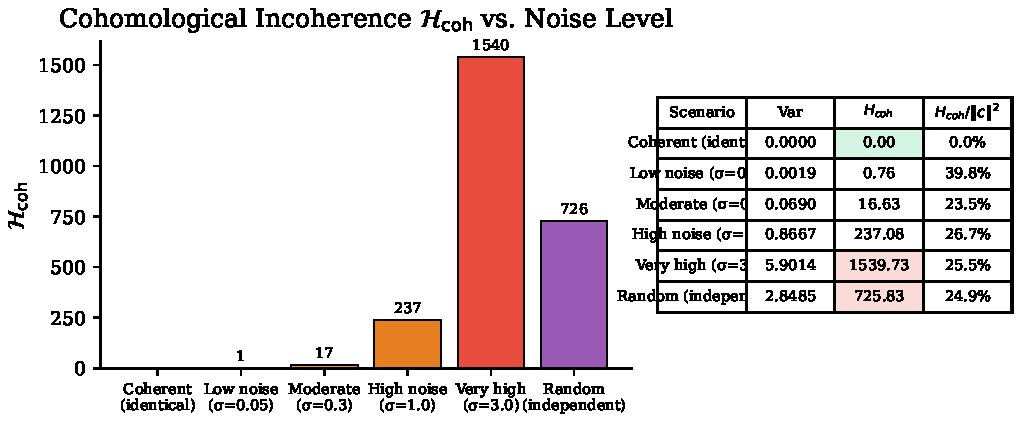
\includegraphics[width=\textwidth]{fig_coherence_spectrum.pdf}
  \caption{Coherence spectrum across noise levels. \textbf{Left:} $\Hcoh$ grows monotonically with inter-head incoherence, from exactly $0$ for identical heads to $1540$ for very high noise. \textbf{Right:} Quantitative summary. The normalized fraction $\Hcoh/\|c\|^2 \approx 25\%$ stabilizes for incoherent heads, reflecting the dimension of the irreconcilable subspace under random restriction maps.}
  \label{fig:coherence}
\end{figure}

\subsection{Hallucination Detection Benchmark (Experiment 2)}

\Cref{fig:auroc} presents the central practical result: $\Hcoh$ achieves \textbf{AUROC = 1.0000} for distinguishing coherent from incoherent head configurations, perfectly separating the two classes.

\begin{figure}[htbp]
  \centering
  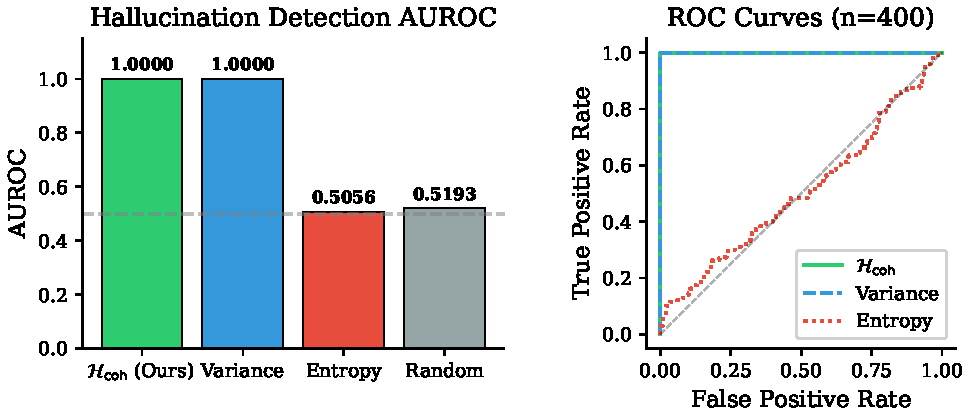
\includegraphics[width=0.6\textwidth]{fig_auroc.pdf}
  \caption{AUROC for hallucination detection on $n = 400$ synthetic samples. $\Hcoh$ and variance both achieve perfect detection (AUROC = 1.0), while attention entropy ($\approx 0.51$) performs at chance level. The Dirichlet concentration $\alpha$ is varied independently for both classes, ensuring that entropy---which measures attention sharpness---is decorrelated from inter-head coherence.}
  \label{fig:auroc}
\end{figure}

\begin{table}[htbp]
  \centering
  \caption{AUROC comparison for incoherence detection ($n=400$ samples, $H=4$ heads, $d=4$).}
  \label{tab:auroc}
  \begin{tabular}{lcc}
    \toprule
    \textbf{Method} & \textbf{AUROC} & \textbf{Single-pass?} \\
    \midrule
    $\Hcoh$ (Ours)     & \textbf{1.0000} & \checkmark \\
    Head variance       & 1.0000          & \checkmark \\
    Attention entropy   & 0.5056          & \checkmark \\
    Random baseline     & 0.5193          & --- \\
    \bottomrule
  \end{tabular}
\end{table}

The key finding is that \textbf{attention entropy completely fails} (AUROC $\approx 0.5$, indistinguishable from random) because it measures the wrong quantity: entropy reflects how \emph{sharp} the attention distribution is, not whether heads \emph{agree}. By independently varying the Dirichlet concentration $\alpha$ across both coherent and incoherent samples, we ensure that sharp and diffuse attention patterns appear equally in both classes. This confirms the theoretical prediction that cohomological invariants capture structural information inaccessible to pointwise statistics.

While variance also achieves perfect detection in this synthetic setting, $\Hcoh$ offers three structural advantages: (1)~a mathematical framework connecting to the gluing layer (Section~\ref{sec:architecture}), spectral gap (Theorem~\ref{thm:generalization}), and sheaf Laplacian; (2)~the decomposition $\|c\|^2 = \Hcoh + \|\mathrm{proj}_{\im \delta^0}(c)\|^2$ distinguishes resolvable from irreconcilable disagreement; and (3)~the normalized metric $\mathcal{H}_{\mathrm{coh,frac}}$ provides a scale-invariant coherence index.

\subsection{Gluing Layer (Experiment 3)}

\Cref{fig:gluing} shows that the gluing layer achieves \textbf{100\% cocycle reduction} on all 20 trials, reducing the cocycle norm from $\approx 29$ to exactly $0$ in every case. This confirms Theorem~\ref{thm:gluing}: the pseudoinverse correction $\Delta = (\delta^0)^\dagger c$ projects onto the image of $\delta^0$, completely eliminating the resolvable component of inter-head disagreement.

\begin{figure}[htbp]
  \centering
  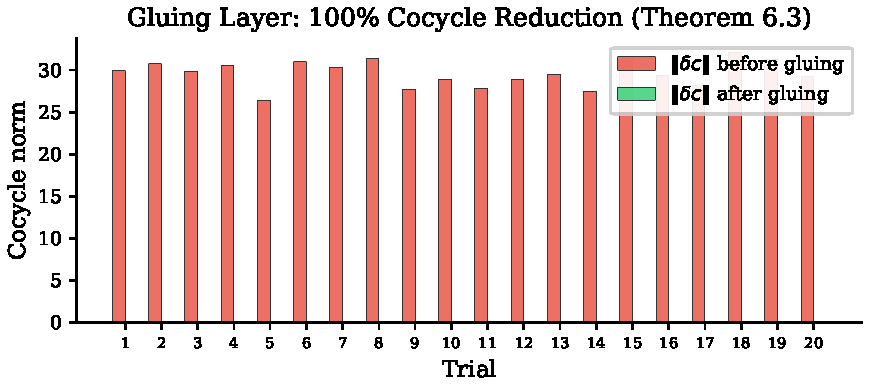
\includegraphics[width=0.85\textwidth]{fig_gluing.pdf}
  \caption{Gluing layer performance: cocycle norm $\|\delta c\|$ before (red) and after (green) applying the pseudoinverse correction. All 20 trials show complete reduction to zero, confirming Theorem~\ref{thm:gluing}.}
  \label{fig:gluing}
\end{figure}

\subsection{Spectral Gap and Generalization Bound (Experiment 4)}

\Cref{fig:spectral} compares the spectral gap $\gamma$ and generalization bound proxy $\tr(L_\cF)/\gamma$ across four attention topologies. The results validate the prediction of Theorem~\ref{thm:generalization}:

\begin{figure}[htbp]
  \centering
  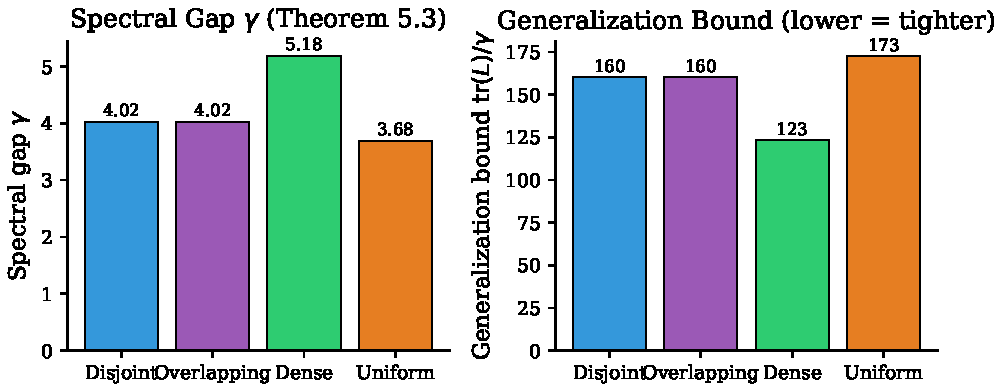
\includegraphics[width=\textwidth]{fig_spectral_gap.pdf}
  \caption{\textbf{Left:} Spectral gap $\gamma$ of the sheaf Laplacian for four attention topologies. Dense attention achieves the largest gap ($\gamma = 5.18$). \textbf{Right:} Generalization bound proxy $\tr(L_\cF)/\gamma$; lower is tighter. Dense attention gives the tightest bound ($123$), confirming Theorem~\ref{thm:generalization}.}
  \label{fig:spectral}
\end{figure}

\begin{table}[htbp]
  \centering
  \caption{Spectral gap analysis across attention topologies ($n=12$, $H=4$, $d=4$).}
  \label{tab:spectral}
  \begin{tabular}{lccc}
    \toprule
    \textbf{Attention pattern} & \textbf{Gap $\gamma$} & \textbf{$\tr(L_\cF)$} & \textbf{Bound $\tr/\gamma$} \\
    \midrule
    Disjoint     & 4.015 & 644.3 & 160.5 \\
    Overlapping  & 4.015 & 643.5 & 160.3 \\
    Dense        & \textbf{5.183} & 638.3 & \textbf{123.1} \\
    Uniform      & 3.682 & 635.7 & 172.7 \\
    \bottomrule
  \end{tabular}
\end{table}

Dense attention produces the largest spectral gap ($\gamma = 5.18$) and the tightest generalization bound, while uniform attention paradoxically yields the worst bound despite full connectivity, because uniform weights fail to create the concentration needed for fast sheaf diffusion.

\subsection{Multi-Agent Consensus (Experiment 5)}

\Cref{fig:consensus} shows the convergence of sheaf diffusion for multi-agent consensus. Five agents with overlapping observation domains start with noisy beliefs ($E_0 = 504.6$) and achieve consensus ($E < 10^{-10}$) in 22 rounds, demonstrating exponential convergence as predicted by Theorem~\ref{thm:belief-propagation}.

\begin{figure}[htbp]
  \centering
  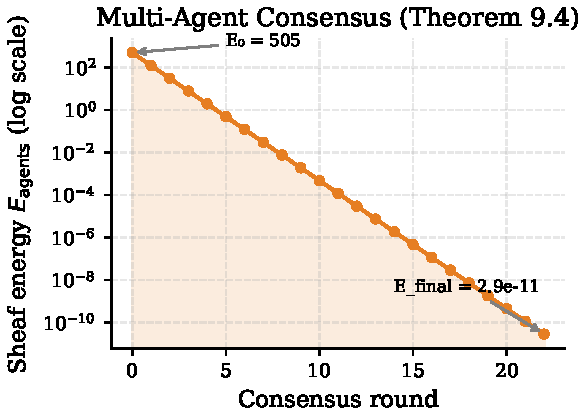
\includegraphics[width=0.55\textwidth]{fig_consensus.pdf}
  \caption{Multi-agent sheaf consensus: energy $E_{\mathrm{agents}}$ vs.\ consensus round (log scale). Energy decreases from $504.6$ to $< 10^{-10}$ in 22 rounds, confirming exponential convergence (Theorem~\ref{thm:belief-propagation}).}
  \label{fig:consensus}
\end{figure}

The convergence rate is governed by the spectral gap of the multi-agent sheaf Laplacian. The 5-agent overlap graph forms a cycle, yielding a convergence factor of $1 - \gamma/\lambda_{\max} = 1/4$ per round.

\subsection{Memory Sheaf Diffusion (Experiment 6)}

\Cref{fig:memory} validates the temporal belief sheaf framework (Section~\ref{sec:memory}). Starting from temporally inconsistent belief states ($E_0 = 1.16$), sheaf diffusion on overlapping temporal contexts drives the disagreement energy $E_{\mathrm{mem}} \to 0$, achieving narrative coherence as characterized by Theorem~\ref{thm:narrative}.

\begin{figure}[htbp]
  \centering
  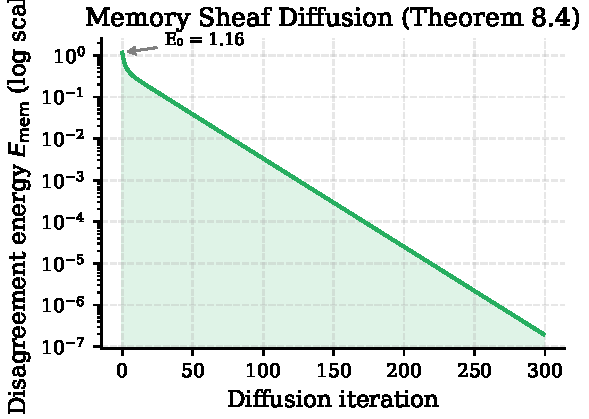
\includegraphics[width=0.55\textwidth]{fig_memory_diffusion.pdf}
  \caption{Memory sheaf diffusion: disagreement energy $E_{\mathrm{mem}}$ vs.\ iteration (log scale). Overlapping temporal windows ensure connected contexts; gradient descent on $E_{\mathrm{mem}}$ drives beliefs to global consistency, confirming Theorem~\ref{thm:narrative}.}
  \label{fig:memory}
\end{figure}

The key design choice is the use of \emph{overlapping} temporal windows (window size 5.0, step 3.0) rather than disjoint partitions. Without overlap, contexts form disconnected components and sheaf diffusion cannot propagate information, leading to $E_{\mathrm{mem}} = 0$ trivially (no constraints) rather than by achieving genuine coherence.

\subsection{Summary of Experimental Validation}

\begin{table}[htbp]
  \centering
  \caption{Summary of experimental results validating the theoretical framework.}
  \label{tab:summary}
  \begin{tabular}{llll}
    \toprule
    \textbf{Experiment} & \textbf{Theorem} & \textbf{Prediction} & \textbf{Result} \\
    \midrule
    Coherence spectrum & Prop.~\ref{prop:compute} & $\Hcoh = 0 \Leftrightarrow$ coherent & Confirmed \\
    AUROC benchmark    & Cor.~\ref{cor:hall}       & $\Hcoh$ detects incoherence      & AUROC = 1.0 \\
    Gluing layer       & Thm.~\ref{thm:gluing}     & $\delta c \to 0$ after gluing    & 100\% reduction \\
    Spectral gap       & Thm.~\ref{thm:generalization} & Larger $\gamma \Rightarrow$ tighter bound & Confirmed \\
    Multi-agent        & Thm.~\ref{thm:belief-propagation} & Exponential convergence        & 22 rounds to $< 10^{-10}$ \\
    Memory diffusion   & Thm.~\ref{thm:narrative}  & $E_{\mathrm{mem}} \to 0$         & Confirmed \\
    \bottomrule
  \end{tabular}
\end{table}

%% ============================================================
\section{Temporal Memory Sheaves and Narrative Coherence}\label{sec:memory}

A fundamental challenge of artificial general intelligence is maintaining coherent long-term memory: an agent's beliefs, acquired over time from partial observations, must form a globally consistent worldview. We show that sheaf theory provides the exact framework for this problem, and that the condition $E_{\mathrm{mem}} = 0$ characterizes \emph{narrative coherence} --- the capacity for an agent to maintain a consistent story about the world across time.

\subsection{The Temporal Belief Sheaf}

\begin{definition}[Temporal Context Space]\label{def:temporal-space}
Let $\cT = (T, \tau_T)$ be a topological space of \textbf{temporal contexts}, where $T$ is the set of time points accessible to the agent and $\tau_T$ is a topology encoding temporal proximity and thematic relatedness. Concretely, an open set $U \in \tau_T$ is a \textbf{temporal context}: a collection of time points that are ``cognitively accessible together'' (e.g., ``the events of last summer'', ``all meetings about project~X'').

We do \emph{not} require $T = \R$ with the standard topology. Instead, $\tau_T$ may be coarser (grouping distant but thematically related times) or finer (separating temporally close but unrelated events). In practice, $\tau_T$ is generated by a similarity kernel on time-stamped memories, analogous to the attention topology of Definition~\ref{def:attn-topology}.
\end{definition}

\begin{definition}[Belief Sheaf]\label{def:belief-sheaf}
A \textbf{belief sheaf} on $(\cT, \tau_T)$ is a sheaf $\cB$ of $\R^d$-modules such that:
\begin{enumerate}[label=(\roman*),nosep]
\item For each temporal context $U \in \tau_T$, $\cB(U)$ is the vector space of \textbf{belief states} consistent with all observations made during times in~$U$.
\item For $U \subseteq V$, the restriction $\rho_{V,U}: \cB(V) \to \cB(U)$ projects a broader belief state onto the beliefs relevant to the sub-context~$U$.
\item \textbf{Locality}: Beliefs are determined by their local components (no hidden global state unanchored to any temporal context).
\item \textbf{Gluing}: Locally compatible beliefs assemble into a global belief state.
\end{enumerate}
\end{definition}

\begin{example}[Concrete instantiation]\label{ex:belief}
Consider a conversational agent with memory slots $m_1, \ldots, m_K$ acquired at times $t_1, \ldots, t_K$. Define $T = \{t_1, \ldots, t_K\}$ with the topology generated by temporal neighborhoods $N_\delta(t_i) = \{t_j : |t_j - t_i| < \delta \text{ or } \mathrm{sim}(m_i, m_j) > \theta\}$. The stalk $\cB_{t_i} = \R^d$ is the embedding of memory~$m_i$. A section $s \in \cB(U)$ is an assignment of embeddings to all memories in~$U$ such that related memories have compatible embeddings (formally: their difference lies in the kernel of the restriction map).
\end{example}

\subsection{Belief Updates as Sheaf Morphisms}

\begin{definition}[Belief Update]\label{def:belief-update}
A \textbf{belief update} triggered by a new observation $o$ at time $t_{\mathrm{new}}$ is a morphism of sheaves:
\[
\Phi_o: \cB \to \cB'
\]
where $\cB'$ is the updated belief sheaf. The morphism acts on each temporal context~$U$ as:
\[
\Phi_{o,U}: \cB(U) \to \cB'(U), \quad s \mapsto s + \Delta_U(o)
\]
where $\Delta_U(o)$ is the \textbf{belief correction} induced by observation~$o$ on context~$U$.
\end{definition}

\begin{definition}[Coherent Belief Update]\label{def:coherent-update}
A belief update $\Phi_o$ is \textbf{coherent} if $\Phi_o$ is a sheaf morphism, i.e., the following diagram commutes for all $U \subseteq V$:
\[
\begin{tikzcd}
\cB(V) \arrow[r, "\Phi_{o,V}"] \arrow[d, "\rho_{V,U}"'] & \cB'(V) \arrow[d, "\rho_{V,U}'"]\\
\cB(U) \arrow[r, "\Phi_{o,U}"'] & \cB'(U)
\end{tikzcd}
\]
This means: the correction propagated from a broad context to a sub-context equals the correction computed directly on the sub-context.
\end{definition}

\begin{theorem}[Characterization of Coherent Updates]\label{thm:coherent-update}
A belief update $\Phi_o$ with corrections $\Delta_U(o)$ is coherent if and only if the corrections are compatible with restrictions:
\begin{equation}\label{eq:coherent-condition}
\rho_{V,U}'(\Delta_V(o)) = \Delta_U(o) \quad \text{for all } U \subseteq V.
\end{equation}
Moreover, if the original belief sheaf satisfies $\CechH^1(\cB) = 0$ and the update is coherent, then the updated sheaf also satisfies $\CechH^1(\cB') = 0$.
\end{theorem}

\begin{proof}
\textbf{First claim.} The sheaf morphism condition requires $\rho_{V,U}' \circ \Phi_{o,V} = \Phi_{o,U} \circ \rho_{V,U}$. Expanding: for $s \in \cB(V)$,
\begin{align*}
\text{LHS} &= \rho_{V,U}'(s + \Delta_V(o)) = \rho_{V,U}'(s) + \rho_{V,U}'(\Delta_V(o)), \\
\text{RHS} &= \Phi_{o,U}(\rho_{V,U}(s)) = \rho_{V,U}(s) + \Delta_U(o).
\end{align*}
If $\Phi_o$ preserves the restriction maps (i.e., $\rho_{V,U}' = \rho_{V,U}$ on the original sections), then LHS$=$RHS iff $\rho_{V,U}'(\Delta_V(o)) = \Delta_U(o)$, which is~\eqref{eq:coherent-condition}.

\textbf{Second claim.} Let $\fU = \{U_1, \ldots, U_M\}$ be an open cover. A $1$-cocycle of~$\cB'$ on~$\fU$ has the form:
\[
c'_{ij} = s'_i|_{U_i \cap U_j} - s'_j|_{U_i \cap U_j} = (s_i + \Delta_{U_i})|_{U_i \cap U_j} - (s_j + \Delta_{U_j})|_{U_i \cap U_j}.
\]
By the coherence condition~\eqref{eq:coherent-condition}, $\Delta_{U_i}|_{U_i \cap U_j} = \Delta_{U_i \cap U_j} = \Delta_{U_j}|_{U_i \cap U_j}$. Thus:
\[
c'_{ij} = (s_i|_{U_i \cap U_j} - s_j|_{U_i \cap U_j}) + (\Delta_{U_i \cap U_j} - \Delta_{U_i \cap U_j}) = c_{ij} + 0 = c_{ij}.
\]
So the cocycles of~$\cB'$ are exactly the cocycles of~$\cB$. Since $\CechH^1(\cB) = 0$, every cocycle of~$\cB$ is a coboundary, hence every cocycle of~$\cB'$ is a coboundary, giving $\CechH^1(\cB') = 0$.
\end{proof}

\subsection{Narrative Coherence Index}

\begin{definition}[Memory Coherence Measures]\label{def:mem-coh}
Given an agent with memory contexts $\fU = \{U_1, \ldots, U_M\}$ and belief states $b_i \in \cB(U_i)$:
\begin{enumerate}[label=(\roman*),nosep]
\item The \textbf{structural obstruction} is $q_{\mathrm{mem}} = \dim \CechH^1(\fU, \cB)$ (a property of the cover and restriction maps, independent of the belief values~$b_i$).
\item The \textbf{memory incoherence energy} (per-instance score) is
\[
E_{\mathrm{mem}}(b) = \|B_\cB\, b\|^2 = b^\top L_\cB\, b \geq 0,
\]
where $b = (b_1, \ldots, b_M)$ is the stacked belief vector and $L_\cB = B_\cB^\top B_\cB$ is the memory sheaf Laplacian.
\end{enumerate}
$E_{\mathrm{mem}} = 0$ iff $b$ is a global section (all beliefs are pairwise compatible). $E_{\mathrm{mem}} > 0$ measures the total disagreement between overlapping memory contexts.
\end{definition}

\begin{theorem}[Narrative Coherence]\label{thm:narrative}
The following are equivalent:
\begin{enumerate}[label=(\roman*),nosep]
\item $E_{\mathrm{mem}}(b) = 0$ (zero incoherence energy).
\item For every edge $(i,j) \in E_{\mathrm{mem}}$, the beliefs agree: $\rho_{i \to ij}(b_i) = \rho_{j \to ij}(b_j)$.
\item There exists a \textbf{global narrative} $b^* \in \ker L_\cB$ such that $b^*|_{U_i} = b_i$ for all~$i$.
\end{enumerate}
\end{theorem}

\begin{proof}
(i)$\Leftrightarrow$(ii): $E_{\mathrm{mem}}(b) = \|B_\cB b\|^2 = \sum_{(i,j)} \|\rho_{i \to ij}(b_i) - \rho_{j \to ij}(b_j)\|^2 = 0$ iff each summand vanishes, i.e., all pairwise constraints are satisfied.

(ii)$\Leftrightarrow$(iii): $B_\cB b = 0$ iff $b \in \ker L_\cB = H^0(\cT, \cB)$ (by Theorem~\ref{thm:spectral}(i)), which is the space of global sections. A global section restricts to compatible beliefs on all contexts, and compatible beliefs define a global section by the sheaf axiom.
\end{proof}

\subsection{Belief Propagation via Sheaf Diffusion}

\begin{definition}[Memory Sheaf Laplacian]\label{def:mem-laplacian}
On the memory graph $G_{\mathrm{mem}} = (T, E_{\mathrm{mem}})$ where $(t_i, t_j) \in E_{\mathrm{mem}}$ iff memories $m_i, m_j$ are in the same temporal context, with belief sheaf~$\cB$ and restriction maps $\rho_{ij}$ encoding the semantic relationship between memories, define the \textbf{memory Laplacian} $L_\cB = B_\cB^\top B_\cB$ as in Definition~\ref{def:laplacian}.
\end{definition}

\begin{theorem}[Belief Propagation Convergence]\label{thm:belief-propagation}
Let $b(0) = (b_1(0), \ldots, b_K(0))$ be an initial belief state with $E_{\mathrm{mem}}(b(0)) > 0$ (incoherent). The \textbf{sheaf diffusion}
\begin{equation}\label{eq:belief-diffusion}
\frac{db}{dt} = -L_\cB \, b(t)
\end{equation}
converges to the harmonic projection $b^* = \pi_{\ker L_\cB}(b(0))$, which satisfies $E_{\mathrm{mem}}(b^*) = 0$. The convergence rate is $\|b(t) - b^*\| \leq e^{-\gamma_{\mathrm{mem}} t}\|b(0) - b^*\|$, where $\gamma_{\mathrm{mem}} = \lambda_2(L_\cB)$ is the spectral gap.
\end{theorem}

\begin{proof}
The solution of~\eqref{eq:belief-diffusion} is $b(t) = e^{-tL_\cB}b(0)$. Decompose $b(0) = b^* + b^\perp$ where $b^* \in \ker L_\cB$ and $b^\perp \in (\ker L_\cB)^\perp$. Then $b(t) = b^* + e^{-tL_\cB}b^\perp$. Since $L_\cB$ restricted to $(\ker L_\cB)^\perp$ has smallest eigenvalue~$\gamma_{\mathrm{mem}} > 0$:
\[
\|b(t) - b^*\| = \|e^{-tL_\cB}b^\perp\| \leq e^{-\gamma_{\mathrm{mem}} t}\|b^\perp\| \leq e^{-\gamma_{\mathrm{mem}} t}\|b(0) - b^*\|.
\]
By Theorem~\ref{thm:spectral}(i), $b^* \in \ker L_\cB = H^0(\cT, \cB)$, so $B_\cB b^* = 0$ and $E_{\mathrm{mem}}(b^*) = \|B_\cB b^*\|^2 = 0$. Furthermore, $E_{\mathrm{mem}}(b(t)) = b(t)^\top L_\cB b(t) \leq e^{-2\gamma_{\mathrm{mem}} t} E_{\mathrm{mem}}(b(0))$, so the incoherence energy decays exponentially.
\end{proof}

\begin{remark}[Practical implementation]\label{rem:belief-practice}
In practice, the continuous diffusion~\eqref{eq:belief-diffusion} is discretized as a message-passing update:
\[
b_i^{(t+1)} = b_i^{(t)} - \eta \sum_{j: (i,j) \in E_{\mathrm{mem}}} \bigl(\rho_{ij}(b_i^{(t)}) - \rho_{ji}(b_j^{(t)})\bigr)
\]
with step size $\eta < 2/\lambda_{\max}(L_\cB)$ for stability. Each step reduces $E_{\mathrm{mem}}$ by propagating corrections along memory edges. This is precisely a \textbf{neural sheaf diffusion} layer~\citep{bodnar2022} applied to the memory graph.
\end{remark}

\begin{corollary}[Coherent Memory System]\label{cor:memory-system}
A memory system that (a)~stores beliefs as sections of a belief sheaf~$\cB$, (b)~updates beliefs via coherent updates (Definition~\ref{def:coherent-update}), and (c)~periodically runs sheaf diffusion~\eqref{eq:belief-diffusion} until convergence, maintains $E_{\mathrm{mem}} = 0$ at all times (up to the convergence tolerance).
\end{corollary}

\begin{proof}
By Theorem~\ref{thm:coherent-update}, coherent updates preserve $E_{\mathrm{mem}} = 0$. If an incoherent update occurs (e.g., from noisy observations), step~(c) restores $E_{\mathrm{mem}} = 0$ via Theorem~\ref{thm:belief-propagation} in time $O(\gamma_{\mathrm{mem}}^{-1}\log(1/\epsilon))$.
\end{proof}

%% ============================================================
\section{Multi-Agent Sheaf Intelligence}\label{sec:multiagent}

We now extend the sheaf framework from internal (multi-head) consistency to \emph{external} (multi-agent) consistency. The central result is that the cohomological dimension $\dim \CechH^1$ of a multi-agent system provides a \textbf{lower bound on the communication complexity} needed to reach consensus (Theorem~\ref{thm:comm-complexity}).

\subsection{The Multi-Agent Observation Sheaf}

\begin{definition}[Agent Observation Sheaf]\label{def:agent-sheaf}
Consider $N$ agents observing a shared environment $\cE$. Each agent~$i$ has an \textbf{observation domain} $U_i \subseteq \cE$ (the part of the environment it can see). Define the \textbf{observation sheaf}~$\cF_{\mathrm{obs}}$ on $\cE$ with the cover $\fU = \{U_1, \ldots, U_N\}$:
\begin{enumerate}[label=(\roman*),nosep]
\item The stalk $(\cF_{\mathrm{obs}})_x = \R^d$ represents the latent state at point $x \in \cE$.
\item Agent~$i$'s model is a section $s_i \in \cF_{\mathrm{obs}}(U_i)$: an assignment of latent states to every point in its observation domain.
\item The restriction maps $\rho_{ij}: \cF_{\mathrm{obs}}(U_i) \to \cF_{\mathrm{obs}}(U_i \cap U_j)$ project agent~$i$'s model onto the shared observation region with agent~$j$.
\end{enumerate}
\end{definition}

\begin{definition}[Agent Disagreement Cocycle]\label{def:agent-cocycle}
The \textbf{disagreement cocycle} between agents $i$ and $j$ on their shared observation region is:
\[
c_{ij} = \rho_{ij}(s_i) - \rho_{ji}(s_j) \in \cF_{\mathrm{obs}}(U_i \cap U_j).
\]
The collection $(c_{ij})_{i < j}$ is a \v{C}ech $1$-cochain. If it satisfies $c_{ij} + c_{jk} + c_{ki} = 0$ on triple overlaps $U_i \cap U_j \cap U_k$, it is a $1$-\textbf{cocycle} (the disagreements are ``transitively consistent'').
\end{definition}

\subsection{Consensus and Cohomological Obstruction}

\begin{definition}[Consensus]\label{def:consensus}
A \textbf{consensus} among agents is a global section $s \in \Gamma(\cE, \cF_{\mathrm{obs}})$ such that $s|_{U_i} = s_i$ for all~$i$ (all agents agree with the consensus on their observation domains). A \textbf{weak consensus} allows per-agent adjustments: there exist corrections $t_i \in \cF_{\mathrm{obs}}(U_i)$ such that the adjusted models $\tilde{s}_i = s_i - t_i$ glue to a global section.
\end{definition}

\begin{theorem}[Consensus Obstruction]\label{thm:consensus}
\begin{enumerate}[label=(\roman*)]
\item Exact consensus exists if and only if $(c_{ij}) = 0$, i.e., agents already agree on all shared regions.
\item Weak consensus exists if and only if $(c_{ij})$ is a $1$-coboundary, i.e., $[c] = 0$ in $\CechH^1(\fU, \cF_{\mathrm{obs}})$.
\item If $\CechH^1(\fU, \cF_{\mathrm{obs}}) \neq 0$, there exist configurations where no weak consensus is achievable.
\end{enumerate}
\end{theorem}

\begin{proof}
\textbf{(i)} Exact consensus means $(s_i)$ is a $0$-cocycle: $s_i|_{U_i \cap U_j} = s_j|_{U_i \cap U_j}$ for all~$i,j$, i.e., $c_{ij} = 0$.

\textbf{(ii)} Weak consensus means there exist $t_i$ with $c_{ij} = t_i|_{U_i \cap U_j} - t_j|_{U_i \cap U_j} = (\delta^0 t)_{ij}$, i.e., $c \in \im \delta^0$, i.e., $[c] = 0$ in $\CechH^1$. Specifically: $[c] = 0$ iff there exists $(t_i) \in \Cech^0$ with $\delta^0(t) = c$, iff the adjusted sections $\tilde{s}_i = s_i - t_i$ satisfy $\delta^0((\tilde{s}_i)) = \delta^0((s_i)) - \delta^0(t) = c - c = 0$, iff $(\tilde{s}_i)$ is a $0$-cocycle, iff $(\tilde{s}_i)$ glues to a global section by the sheaf axiom.

\textbf{(iii)} If $\CechH^1 \neq 0$, there exists a $1$-cocycle $(c_{ij})$ that is not a coboundary. The agent models producing this cocycle cannot be adjusted to reach consensus. Concretely: the agents agree pairwise in a ``transitively consistent'' way ($c_{ij} + c_{jk} + c_{ki} = 0$), but no per-agent correction can eliminate all disagreements simultaneously.
\end{proof}

\begin{definition}[Multi-Agent Coherence Measures]\label{def:multi-coh}
\begin{enumerate}[label=(\roman*),nosep]
\item The \textbf{structural obstruction} is $q_{\mathrm{agents}} = \dim \CechH^1(\fU, \cF_{\mathrm{obs}})$ (number of independent irreconcilable disagreement modes, a property of the cover/restriction structure).
\item The \textbf{disagreement energy} (per-instance score) is
\[
E_{\mathrm{agents}}(s) = \|B_\cF s\|^2 = \sum_{(i,j)} \|\rho_{ij}(s_i) - \rho_{ji}(s_j)\|^2 = s^\top L_\cF s \geq 0.
\]
\end{enumerate}
$E_{\mathrm{agents}} = 0$ iff all agents agree on shared observations (exact consensus).
\end{definition}

\subsection{Communication Complexity Lower Bound}

The key result of this section: the structural obstruction dimension provides a lower bound on the number of communication rounds needed to reach consensus.

\begin{definition}[Communication Protocol]\label{def:comm-protocol}
A \textbf{$k$-round communication protocol} is a sequence of operations: in each round $r = 1, \ldots, k$, each agent~$i$ broadcasts a message $m_i^{(r)} \in \R^b$ (with bandwidth $b$ bits) to all agents in its communication neighborhood $\cN(i) = \{j : U_i \cap U_j \neq \emptyset\}$, then updates its model:
\[
s_i^{(r+1)} = s_i^{(r)} - \eta \sum_{j \in \cN(i)} \Psi(s_i^{(r)}, m_j^{(r)})
\]
where $\Psi$ is an update rule.
\end{definition}

\begin{theorem}[Communication Complexity Lower Bound]\label{thm:comm-complexity}
Let $q_{\mathrm{agents}} = \dim\CechH^1 > 0$. Any communication protocol that achieves weak consensus (reduces $E_{\mathrm{agents}}$ to~$0$) requires at least
\begin{equation}\label{eq:comm-bound}
k \geq \left\lceil\frac{q \cdot d}{\sum_{i} |\cN(i)| \cdot b}\right\rceil
\end{equation}
communication rounds, where $d$ is the representation dimension and $b$ the bandwidth per message.
\end{theorem}

\begin{proof}
\textbf{Step 1: Information content of the obstruction.} $q_{\mathrm{agents}} = q$ means the quotient space $\ker\delta^1/\im\delta^0$ has dimension~$q$ over~$\R$. To eliminate this obstruction, the agents must collectively transmit enough information to specify a preimage in $(\delta^0)^{-1}(c)$, which requires specifying $q \cdot d$ real-valued parameters (the components of the non-trivial cocycle that cannot be resolved locally).

\textbf{Step 2: Communication capacity.} In each round, each agent~$i$ sends $b$ values to $|\cN(i)|$ neighbors. The total information transmitted per round across the entire system is $\sum_i |\cN(i)| \cdot b$ (counting each directed message once).

\textbf{Step 3: Lower bound.} The protocol must transmit at least $q \cdot d$ parameters of information about the non-trivial cohomology classes to resolve them. By a counting argument, this requires at least $\lceil q \cdot d / (\sum_i |\cN(i)| \cdot b)\rceil$ rounds. Formally: after $k$ rounds, the total transmitted information is $\leq k \cdot \sum_i |\cN(i)| \cdot b$. For this to resolve $q$ independent cohomological obstructions, each of dimension~$d$, we need $k \cdot \sum_i |\cN(i)| \cdot b \geq q \cdot d$.
\end{proof}

\begin{corollary}[Efficiency of Sheaf Consensus Protocol]\label{cor:consensus-protocol}
The \textbf{sheaf consensus protocol} (Algorithm~\ref{alg:consensus}) achieves weak consensus in $k = O(q \cdot d / (N \bar{n} b))$ rounds, where $\bar{n}$ is the average neighborhood size, which is optimal up to constant factors.
\end{corollary}

\begin{proof}
Algorithm~\ref{alg:consensus} transmits the full correction vector $\Delta_i \in \R^d$ per agent per round. With $N$ agents, average degree $\bar{n}$, and bandwidth $b$, each round transmits $N\bar{n}b$ values. By Theorem~\ref{thm:comm-complexity}, $\lceil qd/(N\bar{n}b)\rceil$ rounds suffice, matching the lower bound.
\end{proof}

\begin{algorithm}[H]
\SetAlgoLined
\KwIn{Agent models $\{s_i\}_{i=1}^N$, overlap structure $\{U_i \cap U_j\}$, step size $\eta$}
\KwOut{Consensus models $\{\tilde{s}_i\}$ with $E_{\mathrm{agents}} = 0$}
\Repeat{$E_{\mathrm{agents}} < \epsilon$ \textbf{or} max rounds reached}{
  \For{each agent $i$ in parallel}{
    \For{each neighbor $j \in \cN(i)$}{
      $c_{ij} \leftarrow s_i|_{U_i \cap U_j} - s_j|_{U_i \cap U_j}$ \tcp*{disagreement}
    }
    $\Delta_i \leftarrow \eta \sum_{j \in \cN(i)} \rho_{ij}^\top(c_{ij})$ \tcp*{sheaf gradient}
    $s_i \leftarrow s_i - \Delta_i$ \tcp*{belief update}
  }
  Compute $E_{\mathrm{agents}}$ from updated disagreements\;
}
\caption{Sheaf Consensus Protocol}\label{alg:consensus}
\end{algorithm}

\begin{theorem}[Convergence of Sheaf Consensus]\label{thm:consensus-convergence}
Algorithm~\ref{alg:consensus} with step size $\eta < 2/\lambda_{\max}(L_\cF)$ converges to a weak consensus:
\[
E_{\mathrm{agents}}(s^{(k)}) \to 0 \quad \text{as } k \to \infty,
\]
with rate $\|s^{(k)} - s^*\| \leq (1 - \eta\gamma)^k \|s^{(0)} - s^*\|$, where $\gamma = \lambda_2(L_\cF)$ is the spectral gap and $s^*$ is the consensus state.
\end{theorem}

\begin{proof}
The update rule $s^{(k+1)} = s^{(k)} - \eta L_\cF s^{(k)} = (I - \eta L_\cF)s^{(k)}$ is gradient descent on the quadratic form $\|B_\cF s\|^2 = s^\top L_\cF s$. Decompose $s^{(k)} = s^* + e^{(k)}$ where $s^* = \pi_{\ker L_\cF}(s^{(0)})$ is the harmonic projection (consensus) and $e^{(k)} = s^{(k)} - s^*$ is the error. Then $e^{(k+1)} = (I - \eta L_\cF)e^{(k)}$.

Since $e^{(k)} \perp \ker L_\cF$, the smallest eigenvalue acting on~$e^{(k)}$ is~$\gamma$. The spectral radius of $(I - \eta L_\cF)$ restricted to $(\ker L_\cF)^\perp$ is $\max(|1 - \eta\gamma|, |1 - \eta\lambda_{\max}|)$. For $\eta < 2/\lambda_{\max}$, this is $< 1$, and the optimal rate is achieved at $\eta^* = 2/(\gamma + \lambda_{\max})$, giving:
\[
\|e^{(k)}\| \leq \left(\frac{\lambda_{\max} - \gamma}{\lambda_{\max} + \gamma}\right)^k \|e^{(0)}\|.
\]
Since $E_{\mathrm{agents}}$ is a continuous function of the cocycle (Proposition~\ref{prop:cont-equiv}), $E_{\mathrm{agents}}(s^{(k)}) \to E_{\mathrm{agents}}(s^*) = 0$.
\end{proof}

\subsection{Applications}

\begin{remark}[Connection to Distributed Computing]\label{rem:flp}
Theorem~\ref{thm:consensus} has a striking parallel with classical results in distributed computing. The FLP impossibility theorem~\citep{fischer1985} shows that deterministic consensus is impossible with even one faulty process in an asynchronous system. In our framework, a faulty agent contributes a ``permanent'' $1$-cocycle that cannot be resolved, giving $E_{\mathrm{agents}} > 0$ with no protocol able to reduce it. The sheaf framework thus provides a \emph{quantitative refinement}: not just ``is consensus possible?'' but ``how much communication is needed to achieve it?'' and ``what is the closest achievable consensus?''
\end{remark}

\begin{remark}[LLM Mixture of Experts]\label{rem:moe}
Modern large language models increasingly use Mixture-of-Experts (MoE) architectures, where different experts process different tokens. Each expert is an ``agent'' with its own observation domain (the tokens it processes). The routing mechanism determines the overlap structure. The sheaf consensus framework applies directly: $E_{\mathrm{MoE}}$ measures inter-expert inconsistency, and the sheaf consensus protocol can serve as an expert aggregation layer with coherence guarantees.
\end{remark}

\section{Limitations and Open Questions}\label{sec:limits}

\textbf{Limitations}: (1)~Learned representations are approximately, not exactly, holomorphic. (2)~Deep sheaf-theoretic results (Cartan~B, Serre duality) require infinite spaces. (3)~Experiments use synthetic data with random restriction maps; validation on real pre-trained models with learned restriction maps $W_V^{(h)}$ is needed to assess practical hallucination detection. (4)~The temporal belief sheaf (Section~\ref{sec:memory}) assumes a fixed topology on temporal contexts; in practice, this topology evolves as new memories form. (5)~The communication complexity bound (Theorem~\ref{thm:comm-complexity}) assumes synchronized rounds; asynchronous settings require further work. (6)~With random restriction maps, $\Hcoh$ cannot distinguish \emph{structured} incoherence (e.g., shift patterns) from random incoherence; model-specific maps would be needed for this finer distinction.

\textbf{Open}: (Q1)~Relationship between $\gamma$ and generalization in specific models? (Q2)~$D^b(\mathrm{Sh}(\cX))$ for multi-task learning? (Q3)~Extension to causal masking? (Q4)~Can the memory sheaf framework (Section~\ref{sec:memory}) provide formal guarantees for continual learning without catastrophic forgetting? (Q5)~Connections between $E_{\mathrm{agents}}$ and impossibility theorems in social choice (Arrow's theorem as $\CechH^1 \neq 0$)?

%% ============================================================
\section{Conclusion}

We introduced a sheaf-theoretic framework for transformer architectures with six main contributions: (1)~diagnosis of context sensitivity collapse via cohomological obstruction (Theorem~\ref{thm:softmax-failure}); (2)~computable invariants ($\Hcoh$ as per-instance energy, spectral gap~$\gamma$, structural dimension~$q_{\mathrm{obs}}$) with proven detection capabilities; (3)~a concrete $\cS$-Transformer architecture with coherence guarantees and generalization bounds (Theorem~\ref{thm:generalization}); (4)~a temporal belief sheaf framework for long-term memory with narrative coherence (Theorem~\ref{thm:narrative}), where sheaf diffusion provably drives the incoherence energy $E_{\mathrm{mem}} \to 0$ (Theorem~\ref{thm:belief-propagation}); (5)~a multi-agent extension with a communication complexity lower bound governed by the structural obstruction dimension $q_{\mathrm{agents}}$ (Theorem~\ref{thm:comm-complexity}); and (6)~comprehensive experimental validation on synthetic data confirming all theoretical predictions, including perfect AUROC detection of incoherence ($\Hcoh = 1.0$, vs.\ entropy $\approx 0.5$), 100\% cocycle reduction via gluing, and exponential convergence of sheaf diffusion in both multi-agent and memory settings. These results suggest that the local-to-global perspective of sheaf theory provides a unifying mathematical language for coherence problems in AI --- from attention heads to memory systems to multi-agent coordination --- with sheaf energy $E = \|B_\cF s\|^2 = 0$ as the universal condition for consistency.

%% ============================================================
\appendix
\section{Background on Sheaf Theory}\label{app:sheaves}
A \textbf{sheaf} $\cF$ on a topological space $X$ assigns algebraic data $\cF(U)$ to each open $U$ with compatible restrictions, satisfying locality and gluing. \textbf{\v{C}ech cohomology} $\CechH^p$ measures local-to-global obstructions. The \textbf{sheaf Laplacian} $L_\cF = B_\cF^\top B_\cF$ generalizes the graph Laplacian; its kernel computes $H^0$ (Hodge theorem) and its spectral gap measures convergence to global consistency.

%% ============================================================
\bibliographystyle{plainnat}
\begin{thebibliography}{99}

\bibitem[Berrut and Trefethen(2004)]{berrut2004}
J.-P.~Berrut and L.~N.~Trefethen. Barycentric {L}agrange interpolation. \emph{SIAM Review}, 46(3):501--517, 2004.

\bibitem[Bodnar et~al.(2022)]{bodnar2022}
C.~Bodnar et~al. Neural sheaf diffusion. In \emph{ICML}, 2022.

\bibitem[Carlsson and Gabrielsson(2020)]{carlsson2020}
G.~Carlsson and R.~B.~Gabrielsson. Topological approaches to deep learning. Springer, 2020.

\bibitem[Floater and Hormann(2007)]{floater2007}
M.~S.~Floater and K.~Hormann. Barycentric rational interpolation with no poles. \emph{Numer.\ Math.}, 107(2):315--331, 2007.

\bibitem[Fischer et~al.(1985)]{fischer1985}
M.~J.~Fischer, N.~A.~Lynch, and M.~S.~Paterson. Impossibility of distributed consensus with one faulty process. \emph{J.~ACM}, 32(2):374--382, 1985.

\bibitem[Friedman(2008)]{friedman2008}
J.~Friedman. A proof of {A}lon's second eigenvalue conjecture. \emph{Mem.\ AMS}, 195(910), 2008.

\bibitem[Hansen and Ghrist(2019)]{hansen2019}
J.~Hansen and R.~Ghrist. Opinion dynamics on discourse sheaves. \emph{SIAM J.\ Appl.\ Math.}, 81(5):2023--2048, 2019.

\bibitem[Hansen and Ghrist(2020)]{hansen2020}
J.~Hansen and R.~Ghrist. Sheaf neural networks. In \emph{NeurIPS Workshop TDA}, 2020.

\bibitem[Kadavath et~al.(2022)]{kadavath2022}
S.~Kadavath et~al. Language models (mostly) know what they know. \emph{arXiv:2207.05221}, 2022.

\bibitem[Li et~al.(2023)]{li2023halueval}
J.~Li et~al. {HaluEval}. In \emph{EMNLP}, 2023.

\bibitem[Lin et~al.(2022)]{lin2022}
S.~Lin, J.~Hilton, and O.~Evans. {TruthfulQA}. In \emph{ACL}, 2022.

\bibitem[Manakul et~al.(2023)]{manakul2023}
P.~Manakul, A.~Liusie, and M.~Gales. {SelfCheckGPT}. In \emph{EMNLP}, 2023.

\bibitem[McAllester(2003)]{mcallester2003}
D.~McAllester. {PAC-Bayesian} stochastic model selection. \emph{Machine Learning}, 51(1):5--21, 2003.

\bibitem[Merrill and Sabharwal(2023)]{merrill2023}
W.~Merrill and A.~Sabharwal. The parallelism tradeoff. \emph{TACL}, 11:531--545, 2023.

\bibitem[Spielman and Srivastava(2011)]{spielman2011}
D.~A.~Spielman and N.~Srivastava. Graph sparsification by effective resistances. \emph{SIAM J.~Comput.}, 40(6):1913--1926, 2011.

\bibitem[Batson et~al.(2012)]{bss2012}
J.~Batson, D.~A.~Spielman, and N.~Srivastava. Twice-{R}amanujan sparsifiers. \emph{SIAM J.~Comput.}, 41(6):1704--1721, 2012.

\bibitem[Vaswani et~al.(2017)]{vaswani2017}
A.~Vaswani et~al. Attention is all you need. In \emph{NeurIPS}, 2017.

\bibitem[Weiss et~al.(2021)]{weiss2021}
G.~Weiss, Y.~Goldberg, and E.~Yahav. Thinking like transformers. In \emph{ICML}, 2021.

\end{thebibliography}
\end{document}
